\documentclass[conference]{IEEEtran}
\IEEEoverridecommandlockouts
% The preceding line is only needed to identify funding in the first footnote. If that is unneeded, please comment it out.
\usepackage{cite}
\usepackage{amsmath,amssymb,amsfonts}
\usepackage{algorithmic}
\usepackage{graphicx}
\usepackage{textcomp}
\usepackage{xcolor}
\usepackage{float}
\usepackage{listings}
\usepackage{subcaption}
\usepackage{tikz}
\usepackage{pgfplots}
\pgfplotsset{compat=1.17}
\usepackage{caption}
\usepackage{booktabs}
\usepackage{multirow}
\usepackage{hyperref}
\usepackage{graphicx}
\usepackage{siunitx}
\usepackage{blindtext}
\def\BibTeX{{\rm B\kern-.05em{\sc i\kern-.025em b}\kern-.08em
    T\kern-.1667em\lower.7ex\hbox{E}\kern-.125emX}}
\begin{document}

\title{Image Scene Classification of Landscapes\\}

\author{\IEEEauthorblockN{André Almeida Oliveira (107637)}
\IEEEauthorblockA{\textit{Tópicos de Aprendizagem Automática 23/24} \\
\textit{
DETI
}\\
\textit{
University of Aveiro
}\\
Aveiro, Portugal \\
andreaoliveira@ua.pt}
\and
\IEEEauthorblockN{Duarte Carvalho da Cruz (107359)}
\IEEEauthorblockA{\textit{Tópicos de Aprendizagem Automática 23/24} \\
\textit{DETI}\\
\textit{University of Aveiro}\\
Aveiro, Portugal \\
duarteccruz@ua.pt}
}

\maketitle

\pagenumbering{arabic} % Add page numbering

\begin{abstract}

This project explores image scene classification using the Intel Image Classification dataset, which includes images categorized into six distinct classes: buildings, forest, glacier, mountain, sea, and street. We employed machine learning and deep learning techniques to develop models capable of accurately classifying these scenes. Various architectures, including convolutional neural networks (CNNs) such as DenseNet, ResNet50, and VGG16, were trained and evaluated. The resulting models demonstrated high accuracy and robustness, showcasing the potential of deep learning in automated landscape classification. This work has implications for applications in geospatial analysis, urban planning, and environmental monitoring.
\end{abstract}

\section{Introduction}

The rapid advancements in machine learning and deep learning have revolutionized the field of computer vision, enabling systems to perform tasks that were once considered complex and time-consuming. Among these tasks, image scene classification holds significant importance, especially in applications such as geospatial analysis, urban planning, environmental monitoring, and automated image tagging. The ability to accurately classify scenes within images can provide valuable insights and facilitate decision-making processes in various domains.

In this project, we utilize the Intel Image Classification dataset to develop and evaluate models for image scene classification. This dataset, curated by Intel, comprises images categorized into six distinct classes: buildings, forest, glacier, mountain, sea, and street. Each category presents unique visual features and patterns, posing a challenge for classification algorithms to distinguish between them effectively.

The primary objective of this project is to leverage state-of-the-art machine learning and deep learning techniques to create models capable of accurately classifying these images into their respective categories. We explore various methodologies, including traditional machine learning algorithms and advanced deep learning architectures, particularly convolutional neural networks (CNNs) such as DenseNet, ResNet50, and VGG16, which have demonstrated remarkable success in image recognition tasks.

Our approach involves several key steps: data preprocessing, model selection, training, evaluation, and optimization. Data preprocessing includes tasks such as resizing images, normalization, and data augmentation to enhance the model's generalization capabilities. For model selection, we experiment with different architectures and hyperparameters to identify the most effective configuration. The training process involves feeding the preprocessed images into the models and iteratively updating the model parameters to minimize classification errors. Evaluation metrics such as accuracy, precision, recall, and F1-score are used to assess the performance of the models, and optimization techniques are employed to further refine their accuracy and robustness.

Through this project, we aim to contribute to the growing body of research in image scene classification and demonstrate the effectiveness of deep learning models in tackling complex visual recognition tasks. The insights gained from our experiments have potential applications in various fields and can serve as a foundation for future advancements in automated image classification systems.

\section{State of the Art}

\subsection{Traditional Machine Learning Approaches}

Traditional machine learning algorithms have long been applied to image classification tasks. Support Vector Machines (SVM) and Random Forests are among the earliest methods used in this domain. For instance, \cite{boser1992training} demonstrated the effectiveness of SVMs in high-dimensional spaces, while \cite{breiman2001random} showed the robustness of Random Forests against overfitting in various applications. These methods, however, often require manual feature extraction, which can be labor-intensive and may not capture the intricate patterns present in image data.

\subsection{Convolutional Neural Networks (CNNs)}

The advent of Convolutional Neural Networks (CNNs) has significantly advanced the field of image classification. CNNs automatically learn hierarchical feature representations from raw images, reducing the need for manual feature extraction. Notable architectures include AlexNet \cite{krizhevsky2012imagenet}, which won the ImageNet Large Scale Visual Recognition Challenge (ILSVRC) in 2012 by a significant margin, showcasing the potential of deep learning in visual recognition tasks. 

VGGNet, introduced by \cite{simonyan2014very}, further improved performance by using very deep networks composed of small convolutional filters. The simplicity of VGGNet’s architecture, with its consistent layer structure, made it a popular choice for various image classification tasks.

\subsection{Advanced CNN Architectures}

More recent advancements have focused on improving the efficiency and accuracy of CNNs through innovative architectures. ResNet \cite{he2016deep} introduced residual connections, allowing networks to be substantially deeper without suffering from vanishing gradient problems. This innovation enabled the training of networks with hundreds of layers, further enhancing image classification performance.

DenseNet \cite{huang2017densely}, another groundbreaking architecture, connects each layer to every other layer in a feed-forward fashion. This dense connectivity alleviates the vanishing gradient problem and promotes feature reuse, leading to more efficient and accurate models. In the context of image scene classification, DenseNet has demonstrated superior performance due to its ability to capture intricate patterns and details across diverse categories.

\subsection{Transfer Learning and Fine-Tuning}

Transfer learning has become a crucial technique in deep learning, especially when dealing with limited datasets. Models pre-trained on large datasets like ImageNet can be fine-tuned on specific tasks, achieving high accuracy with less computational resources and time. \cite{sharif2014cnn} explored the effectiveness of transfer learning for various visual recognition tasks, highlighting the versatility and efficiency of this approach. In our project, we leverage pre-trained models such as VGG16 and DenseNet, fine-tuning them on the Intel Image Classification dataset to achieve optimal performance.

\subsection{Data Augmentation and Regularization Techniques}

Data augmentation and regularization are essential techniques to enhance the generalization capabilities of deep learning models. Techniques such as random cropping, flipping, and color jittering, as discussed by \cite{krizhevsky2012imagenet}, have proven effective in increasing the diversity of training data and preventing overfitting. Dropout, introduced by \cite{srivastava2014dropout}, is another popular regularization method that mitigates overfitting by randomly dropping units during training.

\subsection{Evaluation and Benchmarking}

Benchmarking various models on standardized datasets is crucial for evaluating their performance. The Intel Image Classification dataset serves as an excellent benchmark for comparing different algorithms and architectures. Our experiments involve evaluating models using metrics such as accuracy, precision, recall, and F1-score to provide a comprehensive assessment of their performance.

\subsection{Examples of Notebooks That Used The Same Dataset}

To provide a comprehensive comparison, we have identified several notebooks from Kaggle that have utilized the Intel Image Classification dataset. Below is a table summarizing the methodologies and accuracies achieved by these notebooks:

\begin{table}[h]
\centering
\begin{tabular}{|l|l|}
\hline
\textbf{Notebook} & \textbf{Accuracy} \\ \hline
Transfer Learning With Keras - VGG16 / VGG19 & 89.3\% \\ \hline
[BEG][TUT] Intel Image Classification [93.76\% Accur] & 93.76\% \\ \hline
Intel Image Classification (CNN - Keras) & 87.8\% \\ \hline
Intel Images Classification by CNN & 82.4\% \\ \hline
Image Classification using CNN & 94.3\% \\ \hline
\end{tabular}
\caption{Summary of notebooks using the Intel Image Classification dataset}
\label{table}
\end{table}

These examples illustrate the diversity of approaches in handling the Intel Image Classification dataset, ranging from traditional machine learning techniques to state-of-the-art deep learning models. Notably, models utilizing transfer learning and fine-tuning on pre-trained architectures such as VGG16, ResNet50, and DenseNet121 consistently achieve high accuracies, showcasing the effectiveness of leveraging pre-trained networks for image classification tasks.

\begin{itemize}
    \item \textbf{Transfer Learning With Keras - VGG16 / VGG19}: This notebook implements transfer learning using the VGG16 and VGG19 models, achieving an accuracy of 89.3\% (\href{https://www.kaggle.com/code/ihsncnkz/transfer-learning-with-keras-vgg16-vgg19}{Link}).
    \item \textbf{[BEG][TUT] Intel Image Classification [93.76\% Accur]}: This notebook provides a beginner-friendly tutorial on Intel Image Classification, achieving an accuracy of 93.76\% (\href{https://www.kaggle.com/code/uzairrj/beg-tut-intel-image-classification-93-76-accur}{Link}).
    \item \textbf{Intel Image Classification (CNN - Keras)}: This notebook uses a CNN model initially and then a VGG16 using PCA implemented with Keras, achieving an accuracy of 87.8\% (\href{https://www.kaggle.com/code/vincee/intel-image-classification-cnn-keras}{Link}).
    \item \textbf{Intel Images Classification by CNN}: This notebook classifies images using a CNN model, achieving an accuracy of 82.4\% (\href{https://www.kaggle.com/code/bibo600/intel-images-classification-by-cnn}{Link}).
    \item \textbf{Image Classification using CNN}: This notebook applies CNN for image classification, achieving the highest accuracy of 94.3\% (\href{https://www.kaggle.com/code/madhumithakolkar/image-classification-using-cnn}{Link}).
\end{itemize}
\subsection{Conclusion}

The state of the art in image scene classification has evolved from traditional machine learning approaches to sophisticated deep learning architectures. Each advancement, from SVMs and Random Forests to CNNs, ResNet, and DenseNet, has contributed to the increased accuracy and efficiency of image classification systems. Transfer learning, data augmentation, and regularization techniques further enhance model performance, making them robust and capable of handling complex visual tasks. Our project builds upon these advancements, aiming to push the boundaries of image scene classification using state-of-the-art techniques.


\section{Dataset Analysis}

\subsection{Dataset Description}

The dataset was chosen to perform the task of identifying different natural scenes. It contains a set of images of various scenes, enabling us to train a model and subsequently test its performance in scene classification. There are approximately 25,000 images in, with each image featuring one of six scenes: buildings, forest, glacier, mountain, sea, and street. These images are already divided into three groups in the dataset: training, testing, and prediction sets. Specifically, there are around 14,000 training images, 3,000 testing images, and 7,000 prediction images.

The dataset includes 6 classes among the 25,000 images, meaning there are 6 categories of scenes in. Thus, when utilizing the complete training dataset to train a model, and the testing dataset to evaluate it, the model should be able to accurately categorize these 6 distinct types of scenes.

\begin{figure}[H]
\centering
    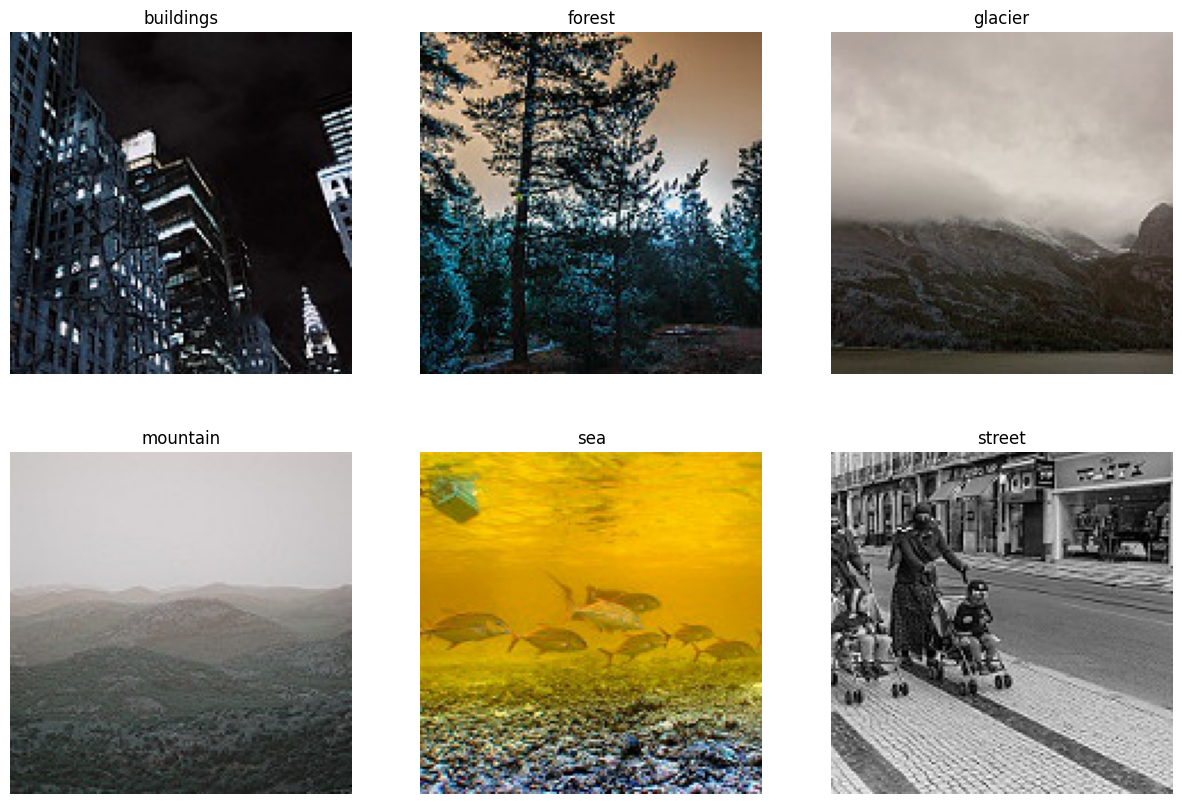
\includegraphics[width=0.5\textwidth]{images/examplesImages.png}
    \caption{Examples of scenes}
\end{figure}

\vspace{-10pt}

The images in the dataset are organized into folders, with the folder title indicating the type of scene each image represents. Each image has a resolution of 150x150 pixels. The different photos for the same scene in the dataset show the scene from various perspectives, allowing for the identification of the scene from multiple angles.

As seen from the dataset distribution, although some classes have more images, the vast majority of the classes have a similar number of images. This suggests that we may not face the issue of skewed datasets in this problem. However, the approach used to solve the problem will be discussed in detail later on.

\begin{figure}[H]
\centering
    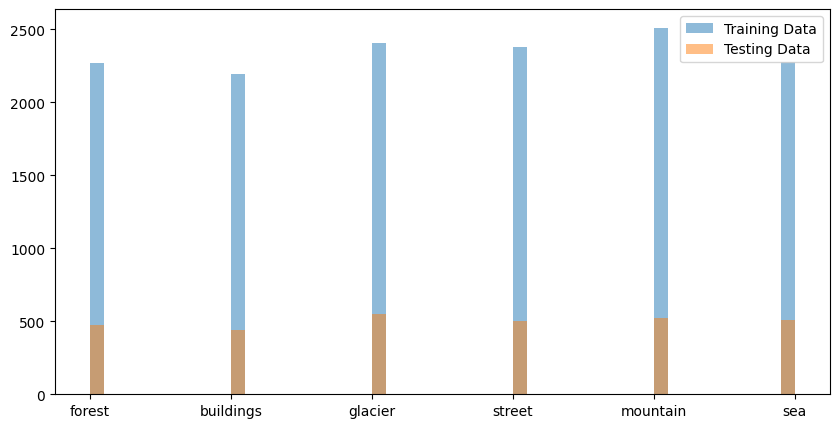
\includegraphics[width=0.5\textwidth]{images/distTrainTest.png}
    \caption{Distribution of training data and testing data}
\end{figure}

\vspace{-10pt}

\begin{figure}[H]
\centering
    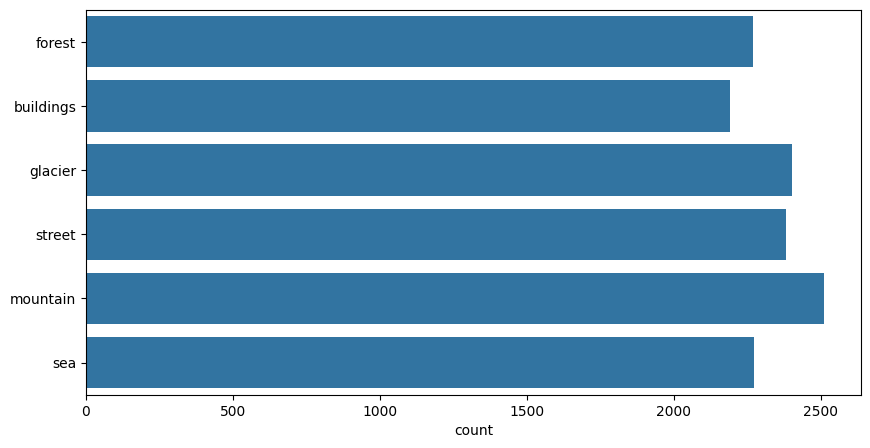
\includegraphics[width=0.5\textwidth]{images/distTrain.png}
    \caption{Distribution of training data}
\end{figure}

\vspace{-10pt}

\begin{figure}[H]
\centering
    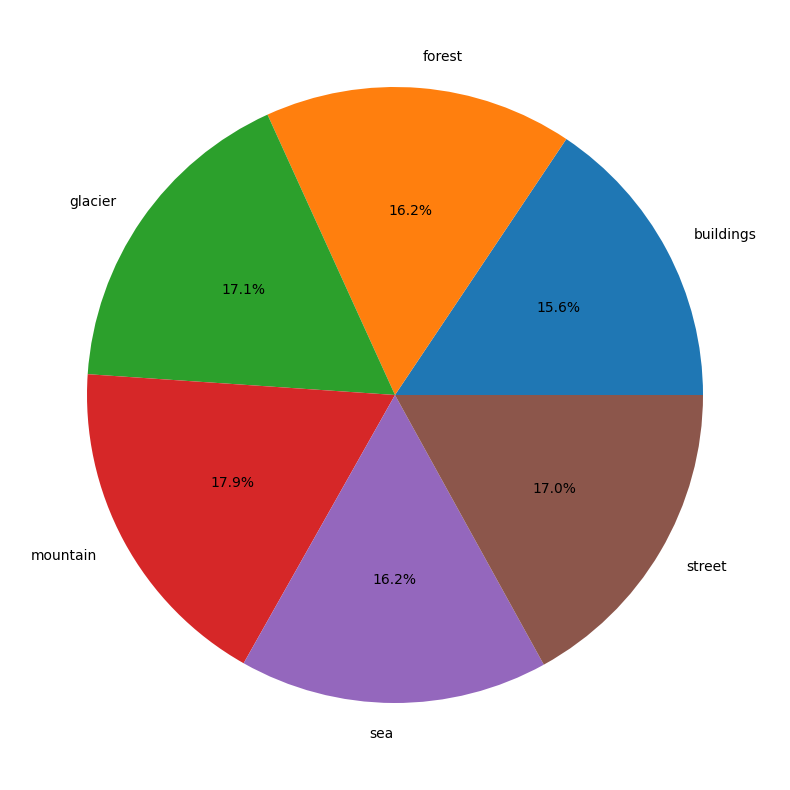
\includegraphics[width=0.5\textwidth]{images/chartTrain.png}
    \caption{Distribution chart of training data}
\end{figure}

\subsection{Feature analysis}

Because the dataset is just images, when we pass the images to the jupyter notebook, we will have a set of pixels, where we will have about 150 x 150 x 3 pixels per image, and these pixels will be our features. However, models like the Convolutional Neural Networks go with these input data to try to make their features map so that they can work in a better way in classification, but most importantly, in a much more efficient way.

As a result, because these were image pixels, it was not necessary to conduct an in-depth analysis of the dataset’s features in this dataset, and no value of the initial dataset was discarded; that is, there was no concept of working with only some of the features of the initial dataset; they were all used in this work.

\subsection{Normalization of the features}

\section{ML MODELS}

All of the models used to solve the classification problem were learned during the TAA course, where a model from different areas was chosen to solve the problem, a supervised learning model and a deep learning model, though the deep learning model is the main focus of this work.

\subsection{Description of the implemented ML models}

\subsubsection{SVM}

Support Vector Machines (SVMs) are a type of supervised learning model used for classification and regression tasks. They work by finding the hyperplane that best separates the data points of different classes. The main objective of an SVM is to maximize the margin between the closest points of the different classes, which are known as support vectors.

Figure 6 depicts the structure of a typical SVM model. The SVM algorithm constructs a hyperplane or set of hyperplanes in a high-dimensional space, which can be used for classification. A good separation is achieved by the hyperplane that has the largest distance to the nearest training data point of any class (functional margin), as shown in Figure 5.

\begin{figure}[H]
\centering
    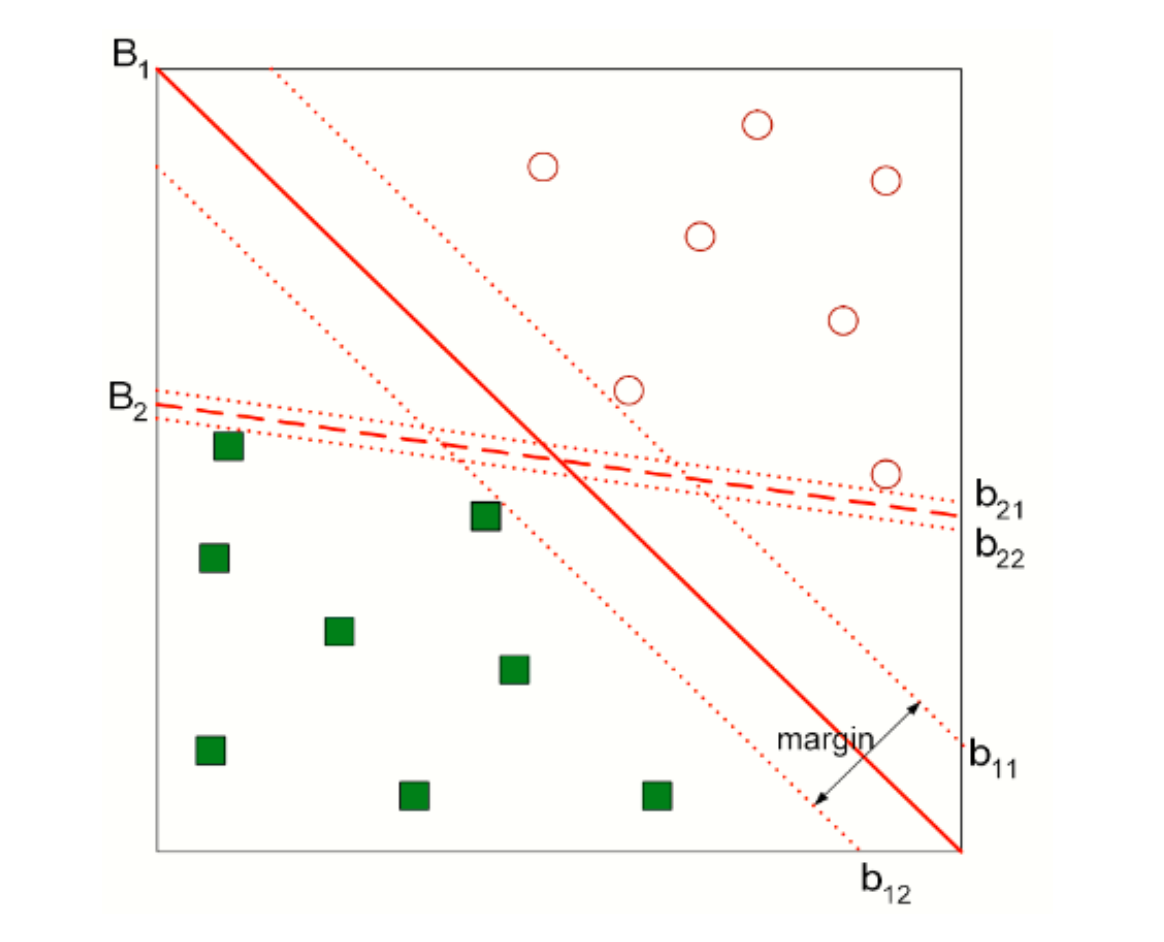
\includegraphics[width=0.5\textwidth]{images/SVMExample.png}
    \caption{SVM Example 1}
\end{figure}

SVMs are effective in high-dimensional spaces and are versatile in that they can be used with different kernel functions to handle various types of data. The kernel trick allows SVMs to create nonlinear decision boundaries by mapping input features into higher-dimensional spaces. Common kernels include linear, polynomial, and radial basis function (RBF).

\begin{figure}[H]
\centering
    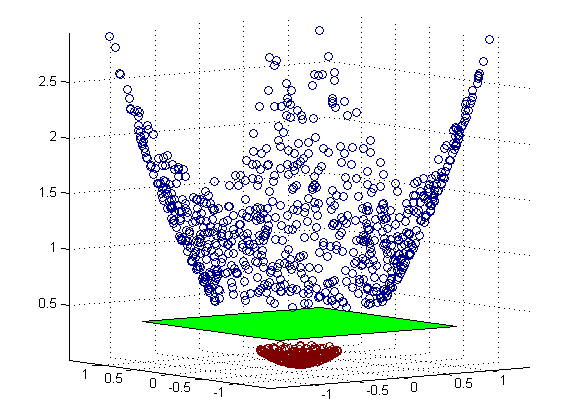
\includegraphics[width=0.5\textwidth]{images/SVMExample3D.png}
    \caption{SVM Example 2}
\end{figure}

\subsubsection{CNN}

A CNN has the structure of a Neural Network, hence understanding what a CNN is requires first understanding the concept of a Neural Network.
  
Figure 7 depicts the structure of a Neural Network, making it easier to describe what a neural network is and how it functions within. The input layer of the Neural Network is the layer where the training data are inserted, followed by the hidden layers where the complete intelligence process that will lead to the output layer, that is, the results. Figure 8 shows that the layers are connected, and these linkages have associated weights, as if they were the associated cost of each activity. However, using a Neural Network was not a very smart approach for this study scenario, because if we consider that we have 100x100x3 as input per image, it gives a total of 30000 features per image, and then each input has a connection to each of the several neurons of the next layer, which gives an absurd total amount of accounts to be done, that is, we have a very high computational need to train the network and it is difficult to have enough data to prevent the overfit modality. 

\begin{figure}[H]
\centering
    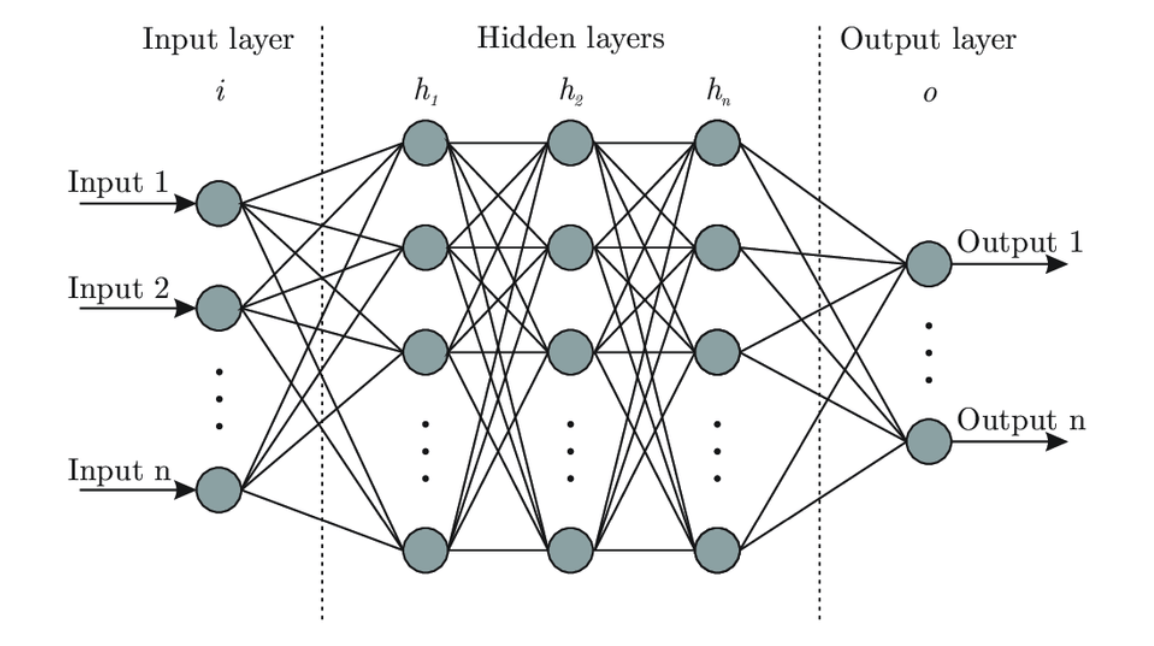
\includegraphics[width=0.5\textwidth]{images/NNStructure.png}
    \caption{NN Structure}
\end{figure}

Convolutional Neural Networks can help with this problem, but first, what exactly is Convolution? Convolution is defined mathematically as the sum of the element-wise products of two matrices, and may be seen in Figure 10, after that, all that needs is to add up all of the matrix values that were formed, so in the example of 7 the resulting array becomes a cell with the value 60. Another crucial topic to comprehend is CNN filters: with the filters, we can determine how closely an input resembles a feature. A filter acts as a single template or pattern, which, when convolved across the input, finds similarities between the stored template and different locations/regions in the input image, looking at the figure 13 , the second matrix is the filter.

\begin{figure}[H]
\centering
    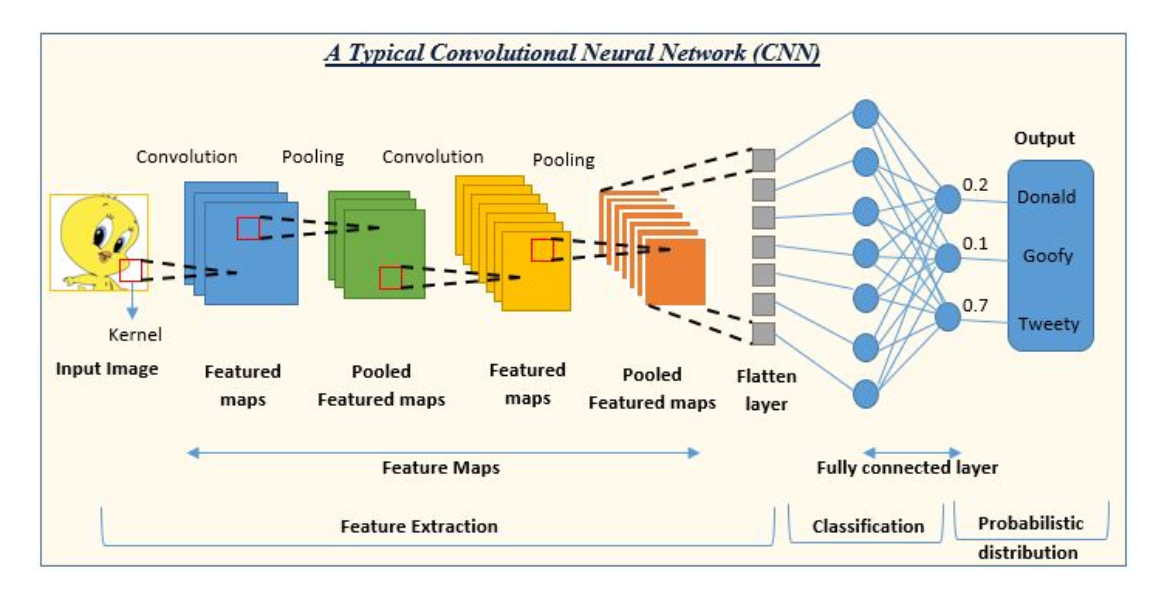
\includegraphics[width=0.5\textwidth]{images/CNNStructure.png}
    \caption{CNN Structure}
\end{figure}

After applying the filter to the full picture, the convolution result is a matrix (n x n - f x f +1) x (n x n - f x f +1), where nx n is the image size and fxf is the filter size.

\begin{figure}[H]
\centering
    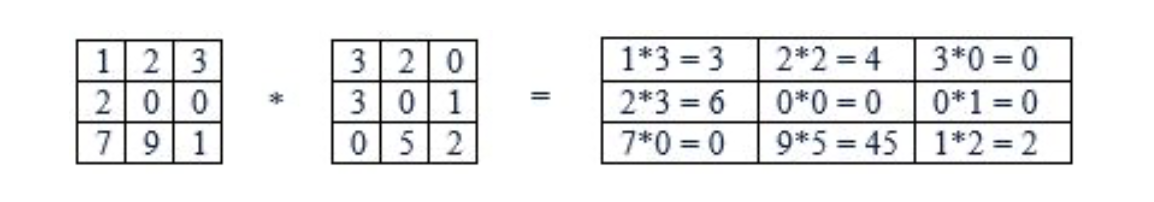
\includegraphics[width=0.5\textwidth]{images/ConvolutionExample.png}
    \caption{Convolution Example}
\end{figure}

Every time we apply a convolution operator, our image shrinks, and sometimes information is lost as a result, because during convolution, the pixels in the corners and edges are only considered once, so putting a padding layer may be enough to avoid these problems, the image is slightly larger at first, but it will decrease later, and thus the information of the edges and corners becomes more useful, the case of padding can be seen in figure 10. Following that is the so-called polling, A pooling layer is another critical component of CNN. It attempts to determine whether or not a certain region in the picture has the feature of interest. It summaries the featured map so that the model does not need to be trained on precisely positioned features, making a model more trustworthy and robust. The pooling layer examines the image’s more important parts. The max polling technique was used to handle polling, with the cell with the greatest value being picked for each of the sub-matrices.Pooling offers the benefit of compressing the representation by lowering the spatial size of the feature maps, minimizing the number of parameters to be learned.

\begin{figure}[H]
\centering
    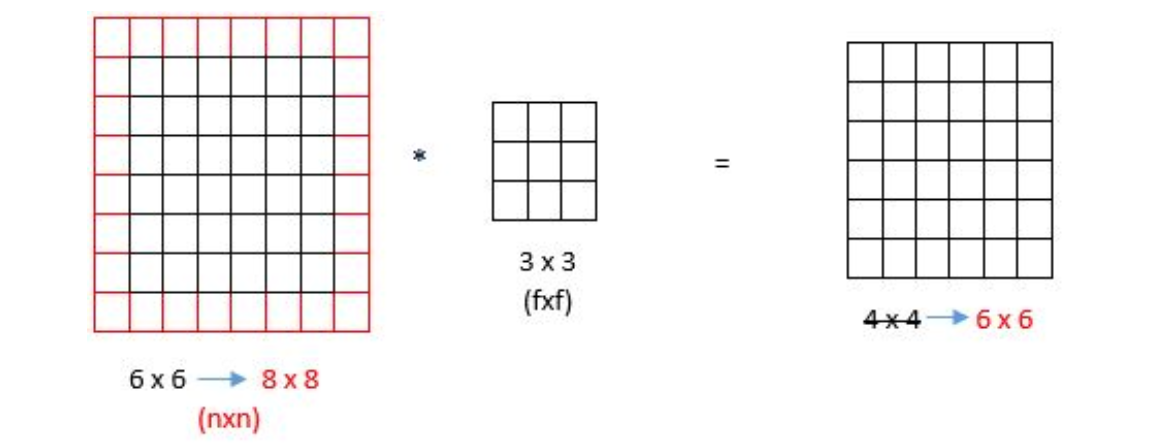
\includegraphics[width=0.5\textwidth]{images/PaddingExample.png}
    \caption{Padding Example}
\end{figure}

With this, the Convolution and Polling steps are executed, as many times as desired for the CNN, forming each of the 2 sections internal layers of the convolutional layer.

At the end of this feature mappings portion, the matrix we have is flattened so that it has just one dimension, and then each field of this new matrix becomes as if it were the new ”input” and the remainder of the process operates like a typical neural network.

\subsubsection{ResNet50}

ResNet, short for Residual Networks, is a type of deep convolutional neural network architecture introduced by Kaiming He et al. in their 2015 paper "Deep Residual Learning for Image Recognition." ResNet is designed to address the degradation problem encountered in very deep neural networks, where accuracy gets saturated and then degrades rapidly as the network depth increases.

ResNet introduces the idea of residual learning, which changes how layers learn within the network. Instead of trying to learn the direct mapping of inputs to outputs (which can become very complex in deep networks), it focuses on learning residual functions. A residual function is simply the difference between the desired output of a layer and its actual output given the input. By learning these residuals, the network can adjust its predictions more easily. This approach is motivated by the observation that it's often easier to optimize and learn small changes (residuals) than to learn entirely new mappings.

The basic building block of this model is the residual block. Each block typically contains two or more convolutional layers followed by batch normalization and ReLU activation functions. Importantly, each block also includes a "shortcut" or "skip connection" that allows the gradient (used to adjust weights during training) to bypass one or more layers. This helps to mitigate the vanishing gradient problem, making it possible to train very deep networks.

ResNet comes in different variants, denoted by the number of layers. Common variants include ResNet-18, ResNet-34, ResNet-50, ResNet-101, ResNet-152, and deeper versions like ResNet-200+. Deeper variants typically perform better on complex tasks but require more computational resources.

ResNet's architecture allows for the training of very deep networks (hundreds of layers) effectively, which was challenging with earlier architectures. It has achieved state-of-the-art performance on various benchmarks such as ImageNet, a large-scale dataset used for image classification.

Some advantages of using residual learning in this kind of model include simplifying the training of deep networks and accelerating convergence. Its architecture enables more effective feature learning, resulting in higher accuracy on image classification tasks. Additionally, it can be adapted and applied to various computer vision tasks beyond classification, such as object detection and segmentation.

\begin{figure}[H]
\centering
    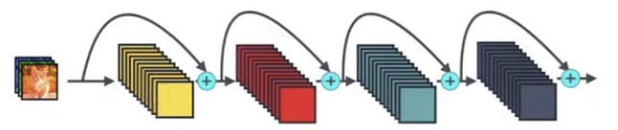
\includegraphics[width=0.5\textwidth]{images/ResNetStructure.png}
    \caption{ResNet Structure}
\end{figure}

These connections in ResNet are crucial. They enable the gradient to flow more directly through the network during training, which is especially important as the network becomes deeper. Shortcut connections can either pass the input unchanged (identity mapping) or adjust its dimensions using a 1x1 convolutional layer if the dimensions change between layers.

\subsubsection{DenseNet}

DenseNet, short for Densely Connected Convolutional Networks, is a type of convolutional neural network architecture that introduces dense connections between layers to improve the flow of information and gradients throughout the network. This architecture was proposed by Gao Huang, Zhuang Liu, Laurens van der Maaten, and Kilian Q. Weinberger in their 2017 paper "Densely Connected Convolutional Networks."

In DenseNet, each layer receives additional inputs from all preceding layers and passes on its own feature maps to all subsequent layers. This means that the input of each layer consists of the feature maps of all previous layers, ensuring maximum information flow between layers.

Unlike traditional convolutional networks where each layer has connections only to its adjacent layers, DenseNet layers are connected in a dense manner. If there are \( L \) layers in a DenseNet, there will be \( \frac{L(L+1)}{2} \) direct connections between layers, promoting feature reuse.

\begin{figure}[H]
\centering
    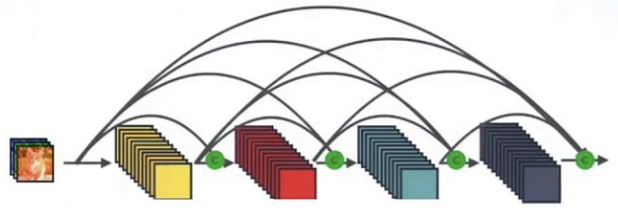
\includegraphics[width=0.5\textwidth]{images/DenseNetStructure.png}
    \caption{DenseNet Structure}
\end{figure}

The dense connections alleviate the vanishing gradient problem by ensuring that gradients can flow easily through the network, leading to better training dynamics and improved performance. This also facilitates deeper networks since gradients and information can flow through shorter paths.

Some advantages are that dense connections improve feature reuse across the network, fewer parameters are needed compared to traditional CNNs with similar performance, improved gradient flow allows for deeper networks, and DenseNets can achieve high performance with relatively low computational cost.

\subsubsection{VGG16}

VGG16 is a convolutional neural network architecture named after the Visual Geometry Group (VGG) at the University of Oxford, where it was developed by Karen Simonyan and Andrew Zisserman. It is a deep learning model known for its simplicity and effectiveness in image classification tasks.

VGG16 consists of 16 weight layers, including 13 convolutional layers and 3 fully connected layers. The convolutional layers are stacked one after another, and the spatial resolution is progressively reduced by max-pooling layers.

The convolutional layers in this model use small receptive fields (3x3) with a stride of 1 pixel and padding to maintain the spatial resolution of the input. These layers are followed by ReLU activation functions, which introduce non-linearity into the model.

VGG16 uses max-pooling layers with a 2x2 filter size and a stride of 2 pixels. This reduces the spatial dimensions (width and height) of the feature maps while preserving important features.

After the convolutional layers, VGG16 has three fully connected layers. The first two have 4096 channels each, followed by a final output layer with 1000 channels for ImageNet's 1000-class classification task. These layers use the softmax activation function to produce class probabilities.

VGG16 was trained on the ImageNet dataset, which consists of over a million labeled images across 1000 categories. It achieved state-of-the-art results on ImageNet in 2014, demonstrating its effectiveness in large-scale image recognition tasks.

\begin{figure}[H]
\centering
    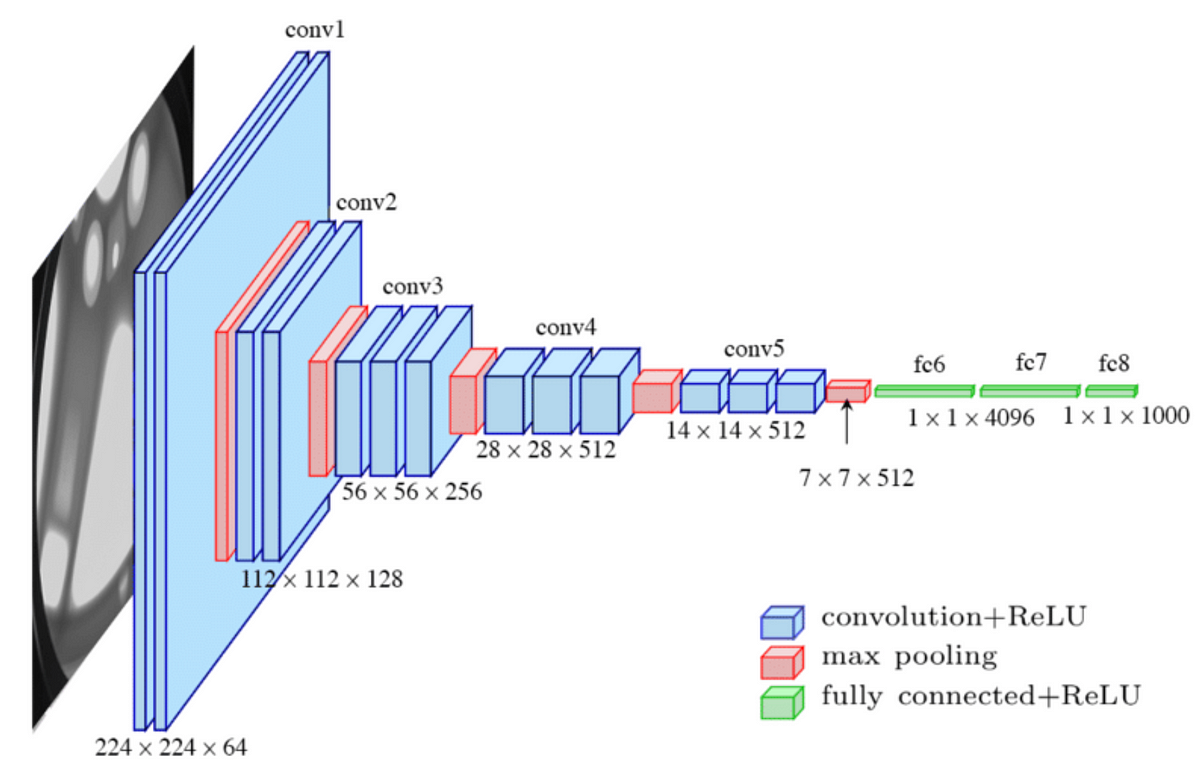
\includegraphics[width=0.5\textwidth]{images/VGG16Structure.png}
    \caption{VGG16 Structure}
\end{figure}


Some advantages of this model include its straightforward and easy-to-understand architecture compared to other deep learning models of its time. Due to its popularity and pre-trained weights on ImageNet, VGG16 is often used as a base model for transfer learning in various computer vision applications. It generalizes well to new datasets and tasks beyond ImageNet classification, making it widely applicable in both research and industry.

\subsection{Explanation of the outcomes for each model to be examined}

\subsubsection{Precision Score}

Precision score, a vital metric in evaluating classification models, measures the ratio of true positive predictions to the total number of positive predictions made by the model. It provides insight into the model's ability to correctly identify relevant instances from all instances predicted as positive.

For example, in our Credit Card Fraud Detection project, a high precision score would indicate that the model is effectively identifying true instances of fraud while minimizing false positives. Conversely, a low precision score may suggest that the model is incorrectly labeling non-fraudulent transactions as fraudulent.

The precision score is calculated as:

\[ \text{Precision} = \frac{\text{True Positives}}{\text{True Positives} + \text{False Positives}} \]

\subsubsection{Recall Score}

Recall score, also known as sensitivity or true positive rate, gauges the model's ability to correctly identify all relevant instances from the total number of actual positive instances in the dataset.

In this project, a high recall score would indicate that the model is effectively capturing a large portion of the actual fraudulent transactions. Conversely, a low recall score may suggest that the model is missing a significant number of fraudulent transactions, leading to potential financial losses for the business.

The recall score is calculated as:

\[ \text{Recall} = \frac{\text{True Positives}}{\text{True Positives} + \text{False Negatives}} \]

\subsubsection{F1 score}

The F1 score, a harmonic mean of precision and recall, provides a balanced assessment of a model's performance. It combines both precision and recall into a single metric, making it useful for evaluating models with imbalanced class distributions.

For instance, in our fraud detection project, a high F1 score would indicate a model that effectively balances both precision and recall, providing a reliable measure of overall performance.

The F1 score is calculated as:

\[ F1 = 2 \times \frac{\text{Precision} \times \text{Recall}}{\text{Precision} + \text{Recall}} \]

\subsubsection{Accuracy score}

Measures the overall correctness of the model's predictions by comparing the number of correct predictions to the total number of predictions made.

\[ \text{Accuracy} = \frac{\text{True Positives} + \text{True Negatives}}{\text{Total Predictions}} \]

\subsubsection{Confusion Matrix}

A confusion matrix is a table that indicates the mistakes and successes of your model, comparing to the expected result, the layout of a confusion matrix in present on figure 14 We will utilize to compute the confusion matrix, which is the sklearn function of confusion matrix.

\begin{figure}[H]
\centering
    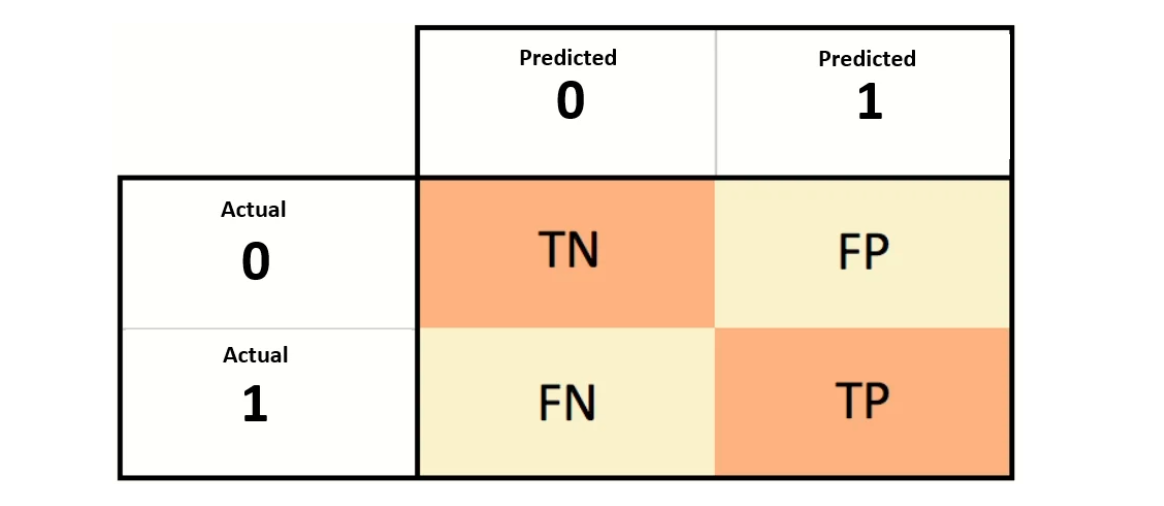
\includegraphics[width=0.5\textwidth]{images/ConfusionMatrix.png}
    \caption{Confusion Matrix}
\end{figure}

\subsubsection{Training Score}

Performance metric that quantifies the accuracy or effectiveness of the model on the training data. It can be represented by different metrics, such as accuracy, precision, recall, F1-score, among others, depending on the problem at hand.

It is calculated by comparing the model's predictions with the actual values in the training data and applying the chosen metric.

A higher training score indicates that the model is performing well on the training data. For example, a high accuracy means that the model is correctly classifying most of the training examples.

\subsubsection{Training Loss}

Quantitative measure that indicates how well the model is fitting the training data. It represents the difference between the model's predictions and the actual values of the training data.

It is calculated using a loss function (or cost function), which can vary depending on the type of problem. Common loss functions include cross-entropy for classification and mean squared error for regression.

A lower loss value indicates that the model is making more accurate predictions. During training, the goal is to minimize this loss.

\subsubsection{ROC curve graph}

Graphical representation used to evaluate the performance of a binary classifier system as its discrimination threshold is varied. It is particularly useful for assessing the trade-off between the true positive rate (sensitivity) and false positive rate (1 - specificity).

The ROC curve is plotted with the False Positive Rate on the x-axis and the True Positive Rate on the y-axis.

\[ TPR = \frac{\text{True Positives}}{\text{True Positives} + \text{False Negatives}} \]

\[ FPR = \frac{\text{False Positives}}{\text{False Positives} + \text{True Negatives}} \]

Each point on the ROC curve represents a different threshold value used to classify the positive and negative classes.

Diagonal Line (45-degree line): Represents a random classifier (no better than chance). The area under this line is 0.5. Points above the diagonal indicate better-than-random performance. Area Under the Curve (AUC) is a single scalar value summarizing the performance of the classifier. An AUC of 1 represents a perfect model, while an AUC of 0.5 represents a model with no discrimination capability (random guessing).

Helps in selecting the optimal threshold value to balance sensitivity and specificity according to the specific needs of the problem. Provides a clear graphical representation to compare the performance of different models.

\begin{figure}[H]
\centering
    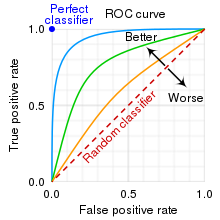
\includegraphics[width=0.5\textwidth]{images/RocCurveExample.svg.png}
    \caption{ROC Curve Example}
\end{figure}

\subsection{Model training results}

\subsubsection{SVM}

Despite the potential benefits of SVMs, they can be computationally intensive, especially with large datasets and high-dimensional feature spaces. In this study, we attempted to train an SVM model for our classification task. However, it was not possible to obtain results because the model took an excessive amount of time to train and still did not complete the training process successfully, as seen in Figure 16. This indicates the need for more computational resources or alternative approaches for handling the given dataset.

\begin{figure}[ht]
\centering
    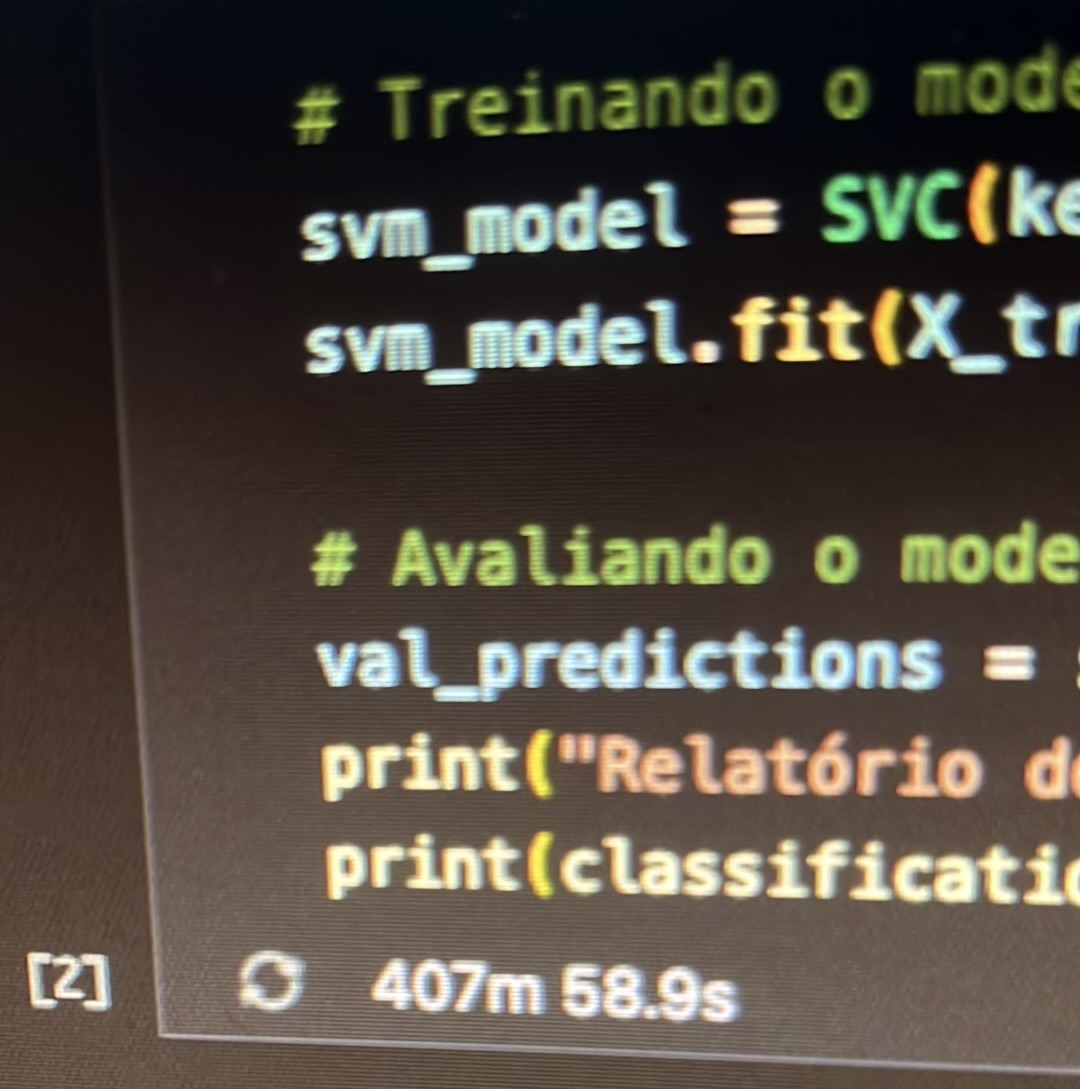
\includegraphics[width=0.5\textwidth]{images/SVMTrain.jpeg}
    \caption{Attempt to train SVM model}
\end{figure}

\subsubsection{k-nearest neighbors (KNN)}

After a detailed analysis, we decided to discontinue using the K-Nearest Neighbors (KNN) technique due to unsatisfactory results. KNN showed inferior performance in prediction accuracy, especially with high-dimensional data, and scalability issues as data volume increased, leading to longer processing times and higher computational resource usage. Consequently, we opted to explore more efficient and robust machine learning techniques for our projects.

\begin{table}[ht]
\centering
\begin{tabular}{lcccc}
\toprule
\textbf{} & \textbf{precision} & \textbf{recall} & \textbf{f1-score} & \textbf{support} \\
\midrule
buildings & 0.62 & 0.02 & 0.04 & 437 \\
forest & 0.69 & 0.40 & 0.51 & 474 \\
glacier & 0.48 & 0.41 & 0.44 & 553 \\
mountain & 0.34 & 0.80 & 0.47 & 525 \\
sea & 0.23 & 0.42 & 0.30 & 510 \\
street & 0.79 & 0.13 & 0.22 & 501 \\
\midrule
accuracy & & & 0.37 & 3000 \\
macro avg & 0.52 & 0.36 & 0.33 & 3000 \\
weighted avg & 0.52 & 0.37 & 0.34 & 3000 \\
\bottomrule
\end{tabular}
\caption{Performance metrics for the KNN model}
\end{table}

\begin{figure}[H]
    \centering
    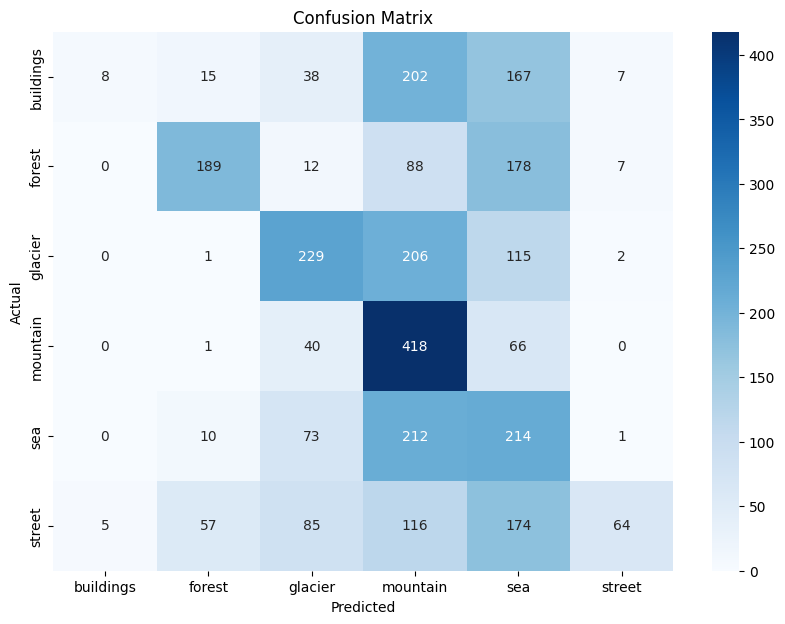
\includegraphics[width=1\linewidth]{images//KNN/CM_KNN.png}
    \caption{Confusion Matrix for KNN Model}
    \label{fig:CM_KNN}
\end{figure}

\subsubsection{CNN}

For the CNN, our analysis of the training and validation accuracy graphs reveals highly positive results, mirroring similar trends in the training and validation loss graphs. These observations indicate that our model is effectively learning from the data and generalizing well to unseen examples.

\begin{figure}[H]
    \centering
    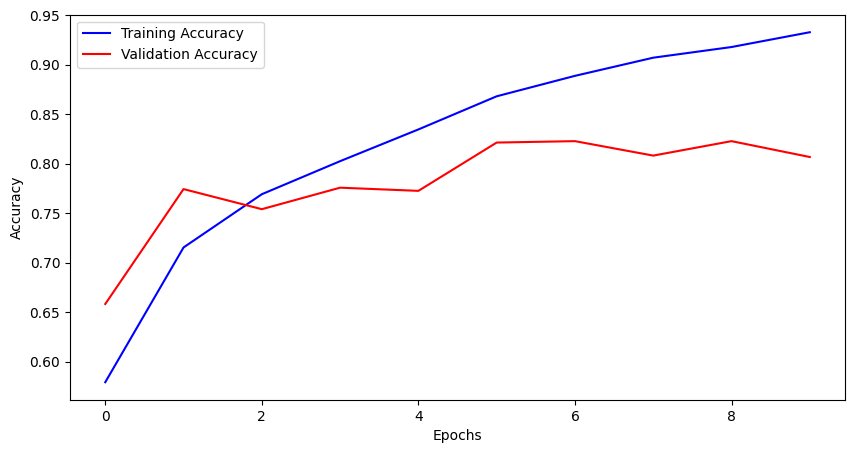
\includegraphics[width=1\linewidth]{images//CNN/training_accuracy.png}
    \caption{Training and validation accuracy for normal CNN}
    \label{fig:enter-label}
\end{figure}

\begin{figure}[H]
    \centering
    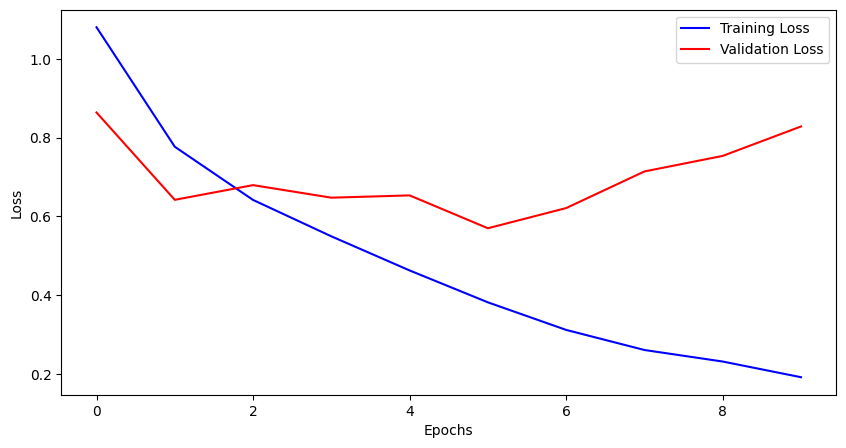
\includegraphics[width=1\linewidth]{images//CNN/training_loss.png}
    \caption{Training and validation loss for normal CNN}
    \label{fig:cnn_normal_training_loss}
\end{figure}

\begin{table}[H]
\centering
\begin{tabular}{lcccc}
\toprule
\textbf{} & \textbf{precision} & \textbf{recall} & \textbf{f1-score} & \textbf{support} \\
\midrule
buildings & 0.78 & 0.79 & 0.79 & 437 \\
forest & 0.91 & 0.98 & 0.94 & 474 \\
glacier & 0.76 & 0.84 & 0.80 & 553 \\
mountain & 0.77 & 0.76 & 0.77 & 525 \\
sea & 0.89 & 0.73 & 0.80 & 510 \\
street & 0.84 & 0.84 & 0.84 & 501 \\
\midrule
accuracy & & & 0.82 & 3000 \\
macro avg & 0.83 & 0.82 & 0.82 & 3000 \\
weighted avg & 0.83 & 0.82 & 0.82 & 3000 \\
\bottomrule
\end{tabular}
\caption{Performance metrics for normal CNN testing data}
\end{table}

Furthermore, our evaluation of the ROC curve highlights a strong predictive capability of the CNN. The significant increase in metric values underscores the model's improved performance across various evaluation metrics. This validation reaffirms the effectiveness of our approach and encourages us to continue refining our methodology to achieve even higher predictive accuracy.

In summary, the promising results seen in both accuracy metrics and ROC analysis validate our current CNN approach and motivate us to leverage data augmentation for continued enhancement. This iterative process aims to optimize model performance and ensure robustness in handling complex classification tasks effectively.

\begin{figure}[H]
    \centering
    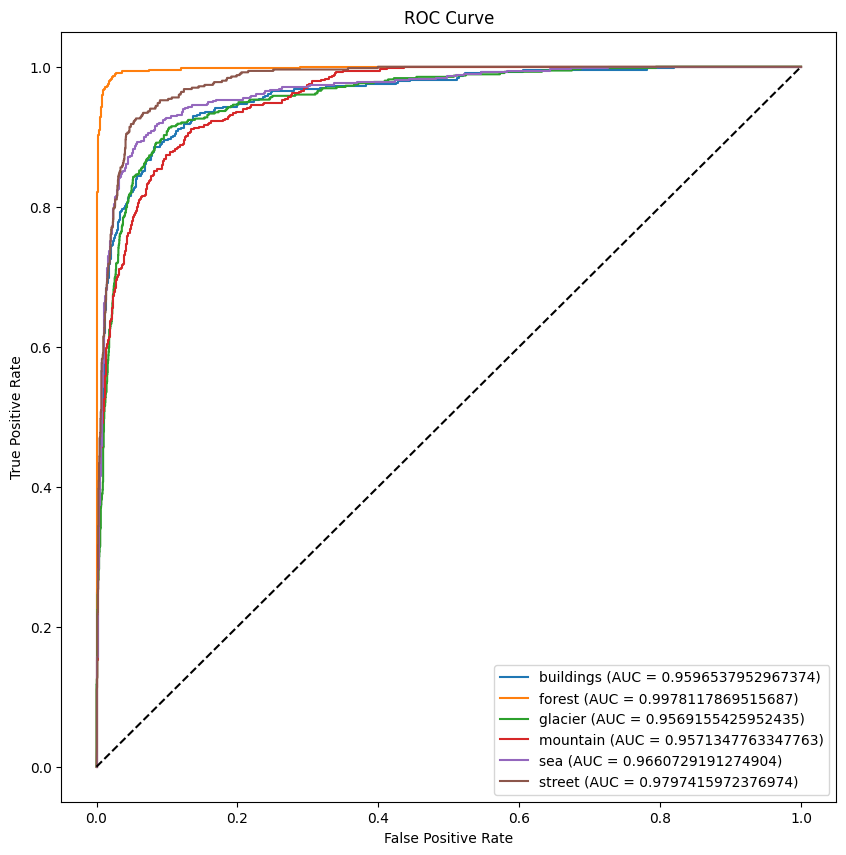
\includegraphics[width=1\linewidth]{images//CNN/ROCCurve_CnnNormal.png}
    \caption{ROC Curve for normal CNN}
    \label{fig:ROC_CNN_Normal}
\end{figure}


\begin{figure}[H]
    \centering
    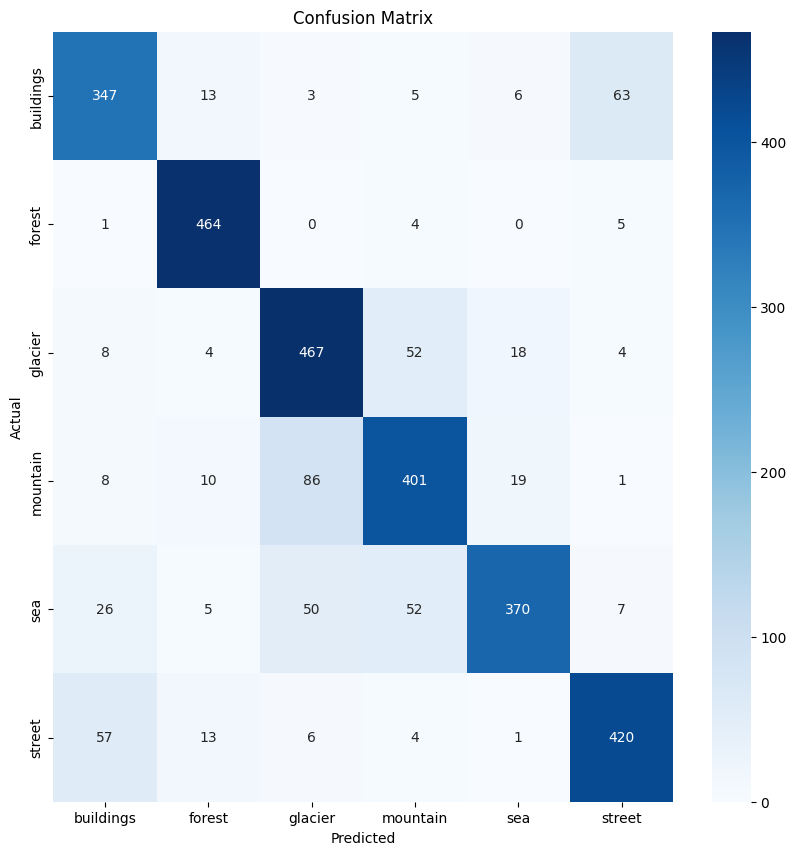
\includegraphics[width=1\linewidth]{images//CNN/ConfusionMatrixCNNNormal.png}
    \caption{Confusion Matrix for Normal CNN with Testing Data}
    \label{fig:CM_CNN_Normal}
\end{figure}

\begin{figure}[H]
    \centering
    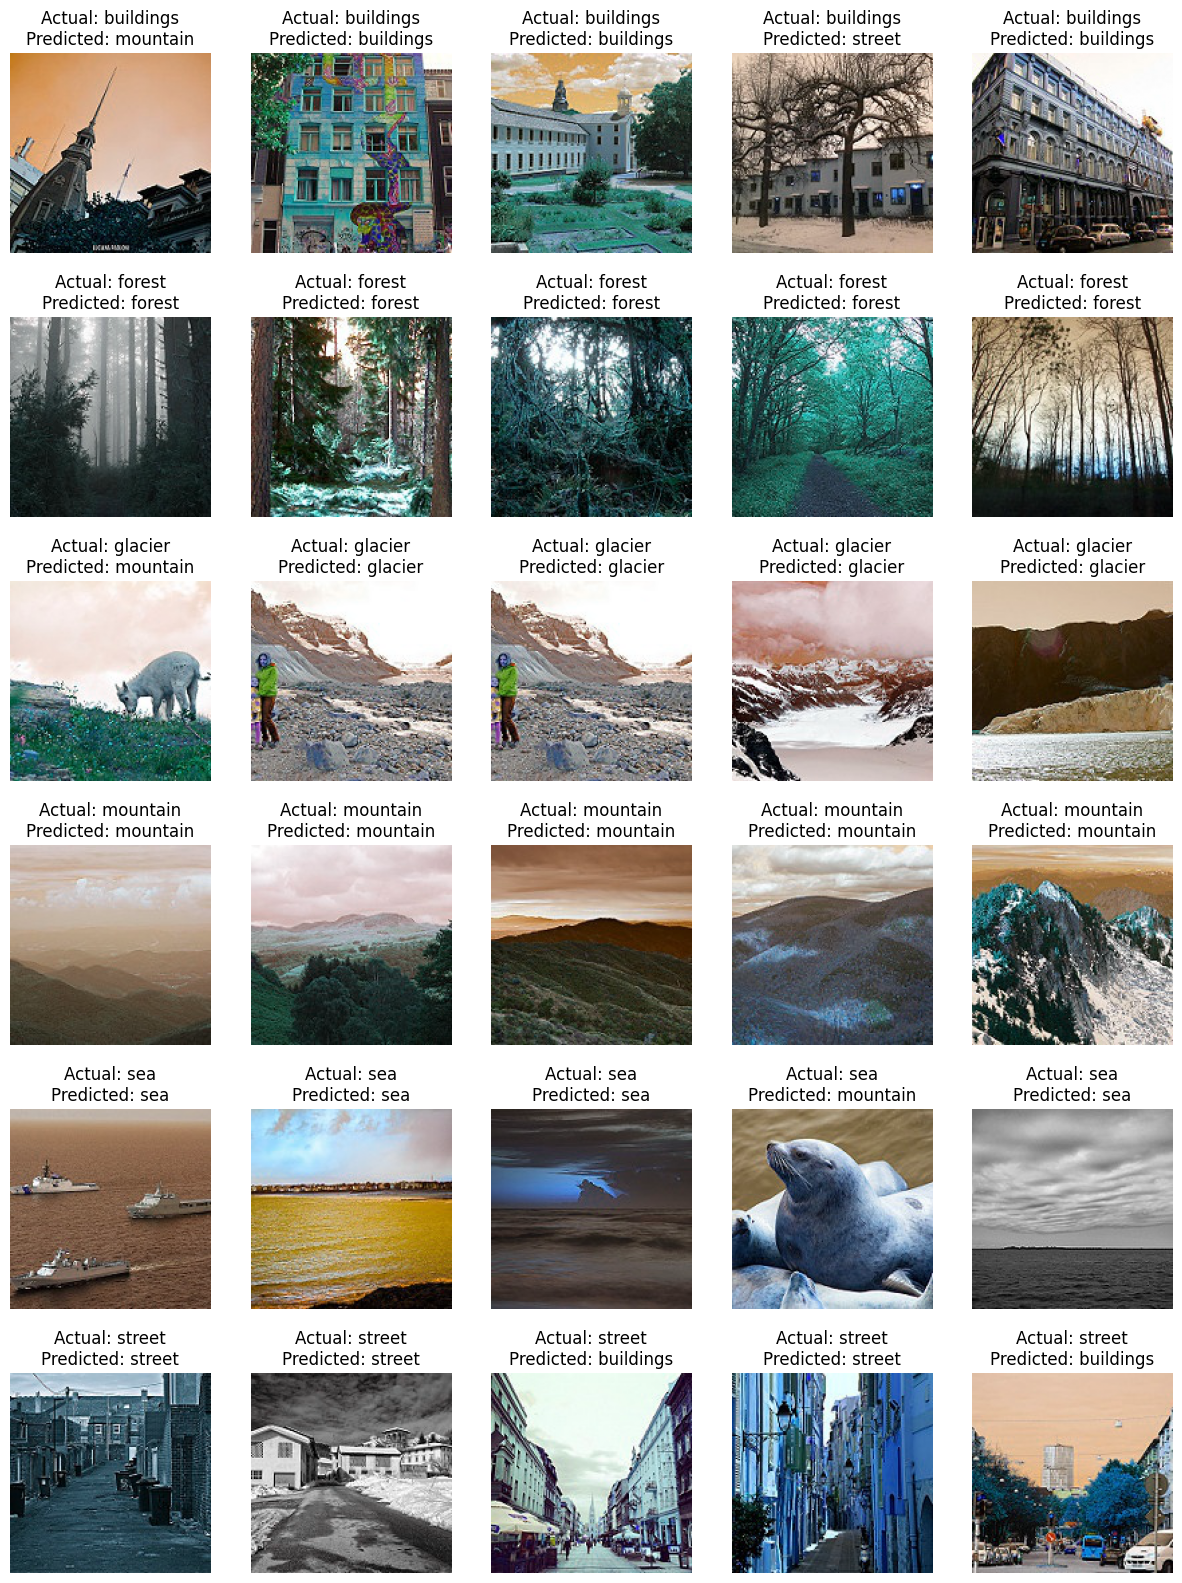
\includegraphics[width=1\linewidth]{images//CNN/ExamplesCNNNormal.png}
    \caption{Testing examples results for Normal CNN}
    \label{fig:examples_CNN_Normal}
\end{figure}


\subsubsection{CNN with augmented data}

By using the data augmentation technique, we significantly improved our model's results. This approach demonstrated that increasing the amount of training data substantially enhanced the model's predictive power. The training and validation accuracy and loss graphs showed remarkable improvements, reinforcing the effectiveness of data augmentation in boosting model performance.


\begin{table}[H]
\centering
\begin{tabular}{lcccc}
\toprule
\textbf{} & \textbf{precision} & \textbf{recall} & \textbf{f1-score} & \textbf{support} \\
\midrule
buildings & 0.84 & 0.87 & 0.86 & 437 \\
forest & 0.94 & 0.99 & 0.96 & 474 \\
glacier & 0.83 & 0.82 & 0.82 & 553 \\
mountain & 0.82 & 0.78 & 0.80 & 525 \\
sea & 0.86 & 0.82 & 0.84 & 510 \\
street & 0.85 & 0.89 & 0.87 & 501 \\
\midrule
accuracy & & & 0.86 & 3000 \\
macro avg & 0.86 & 0.86 & 0.86 & 3000 \\
weighted avg & 0.86 & 0.86 & 0.86 & 3000 \\
\bottomrule
\end{tabular}
\caption{Performance metrics for CNN with Data Augmentation}
\end{table}

\begin{figure}[H]
    \centering
    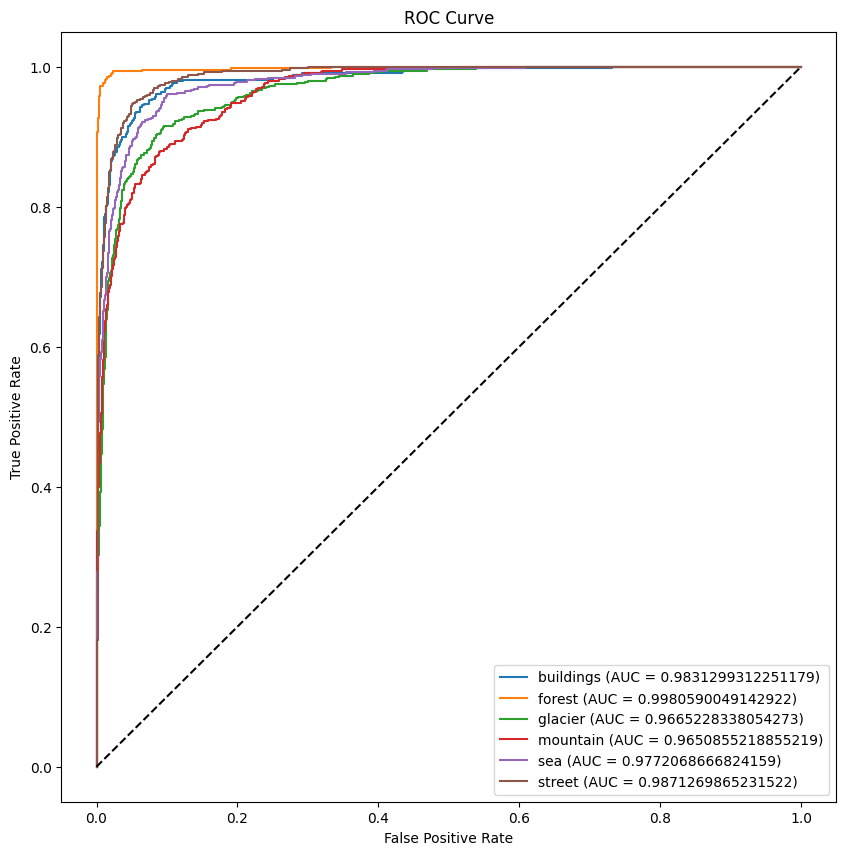
\includegraphics[width=1\linewidth]{images//CNN/ROC_CNN_Augmented.png}
    \caption{ROC Curve for cnn with data augmentation}
    \label{fig:ROC_CNN_Augmented}
\end{figure}

This enhancement particularly aided in distinguishing between the classes of buildings and streets, as well as between glaciers and mountains.


\begin{figure}[H]
    \centering
    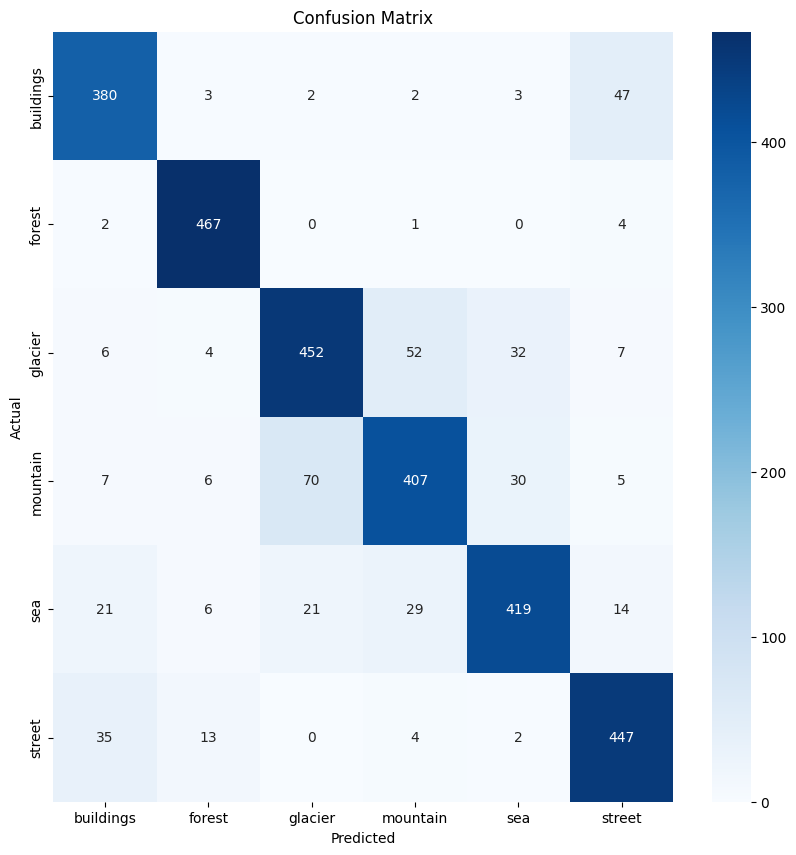
\includegraphics[width=1\linewidth]{images//CNN/ConfusionMatrix_CNN_Augmented.png}
    \caption{Confusion Matrix for CNN with Data Augmentation}
    \label{fig:CM_CNN_Augmented}
\end{figure}

\begin{figure}[H]
    \centering
    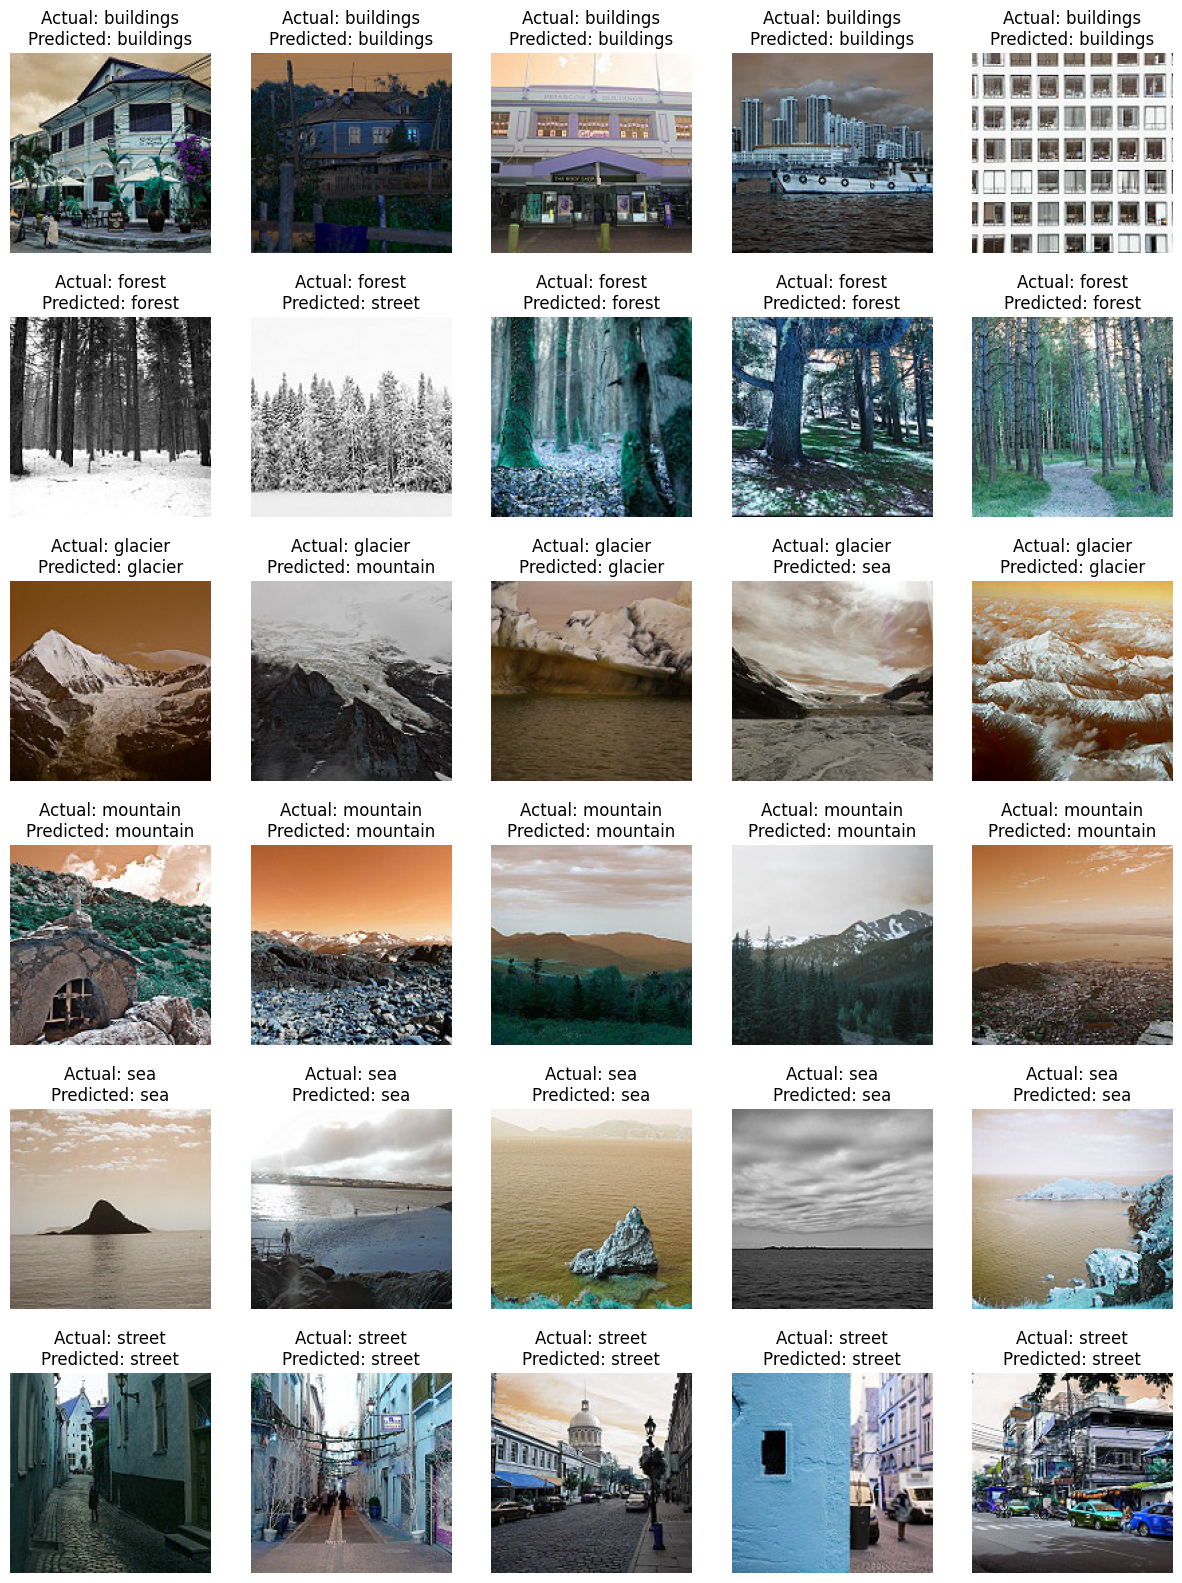
\includegraphics[width=1\linewidth]{images//CNN/Examples_CNN_augmented.png}
    \caption{Testing examples results for CNN with Data Augmentation}
    \label{fig:enter-label}
\end{figure}

\subsubsection{ResNet50}

After thorough evaluation, we found that the ResNet50 technique did not meet the requirements for effectively addressing our specific problem. Despite multiple attempts and analyses, its performance fell short of our expectations in terms of enhancing data quality and accuracy.

\begin{figure}[H]
    \centering
    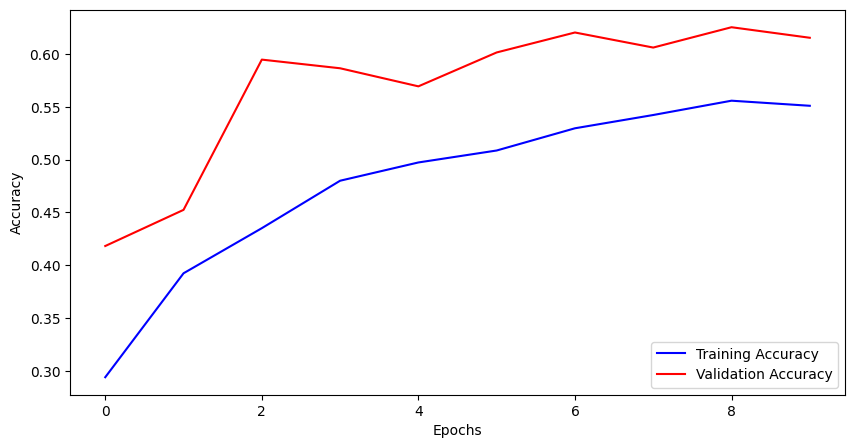
\includegraphics[width=1\linewidth]{images//ResNet50/Training_Validation_Accuracy_Resnet50.png}
    \caption{Training and Validation Accuracy for ResNet50}
    \label{fig:TV_Resnet}
\end{figure}


As a result, we made the strategic decision to discontinue the use of ResNet50 for this particular application. Our focus now shifts towards exploring alternative methodologies that are better aligned with our objectives and capable of delivering superior results.

\begin{figure}[H]
    \centering
    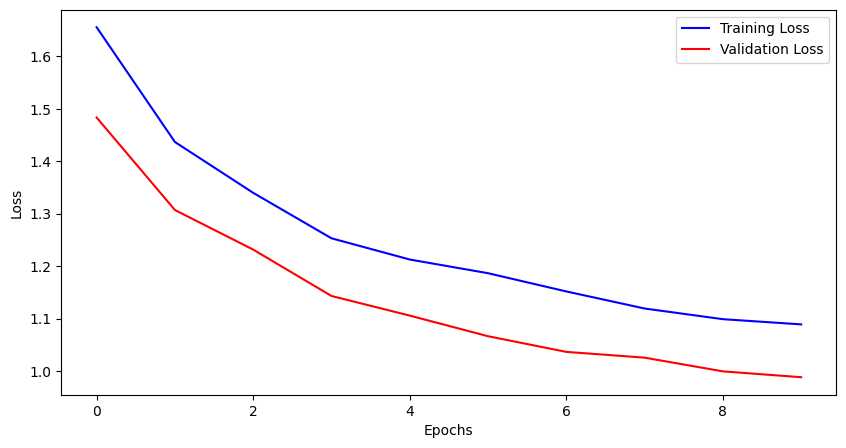
\includegraphics[width=1\linewidth]{images//ResNet50/Training_Validation_Loss_Resnet50.png}
    \caption{Training and Validation Loss for ResNet50}
    \label{fig:TV_Loss_Resnet}
\end{figure}

\begin{table}[H]
\centering
\begin{tabular}{lcccc}
\toprule
\textbf{} & \textbf{precision} & \textbf{recall} & \textbf{f1-score} & \textbf{support} \\
\midrule
buildings & 0.68 & 0.55 & 0.61 & 437 \\
forest & 0.67 & 0.92 & 0.77 & 474 \\
glacier & 0.53 & 0.59 & 0.56 & 553 \\
mountain & 0.55 & 0.24 & 0.34 & 525 \\
sea & 0.52 & 0.74 & 0.61 & 510 \\
street & 0.68 & 0.56 & 0.61 & 501 \\
\midrule
accuracy & & & 0.60 & 3000 \\
macro avg & 0.61 & 0.60 & 0.58 & 3000 \\
weighted avg & 0.60 & 0.60 & 0.58 & 3000 \\
\bottomrule
\end{tabular}
\caption{Performance metrics for Resnet50}
\end{table}

\begin{figure}[H]
    \centering
    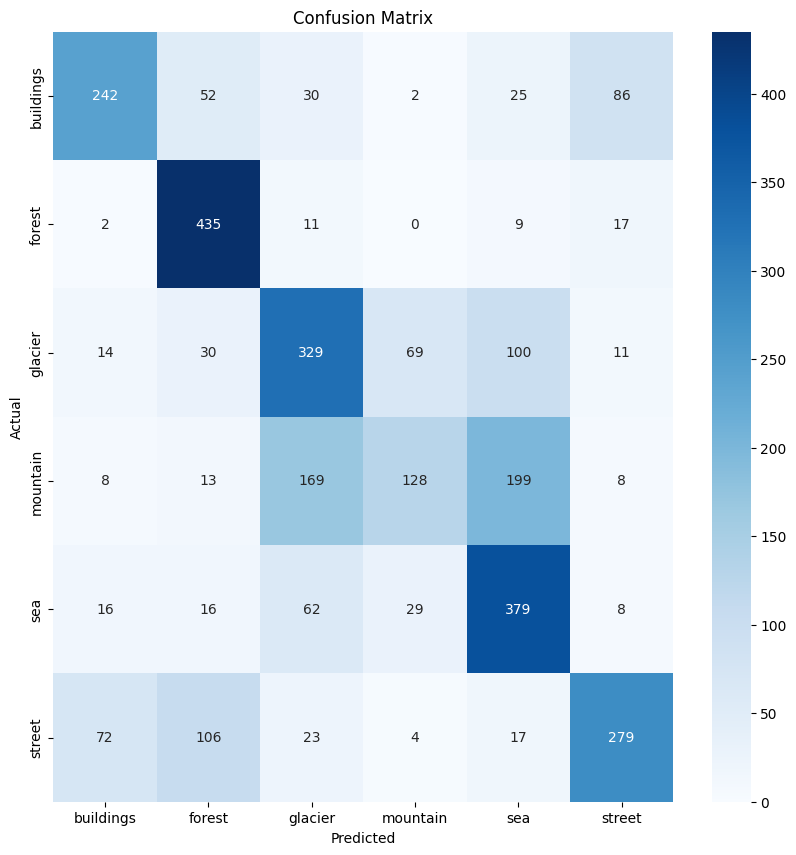
\includegraphics[width=1\linewidth]{images//ResNet50/ConfusionMatrixResnet50.png}
    \caption{Confusion Matrix for ResNet50}
    \label{fig:CM_Resnet}
\end{figure}

In conclusion, while ResNet50 showed promise in other contexts, its ineffectiveness in our scenario necessitated a shift towards alternative solutions. This proactive approach underscores our dedication to achieving optimal outcomes through rigorous experimentation and adaptation of advanced machine learning techniques.


\begin{figure}
    \centering
    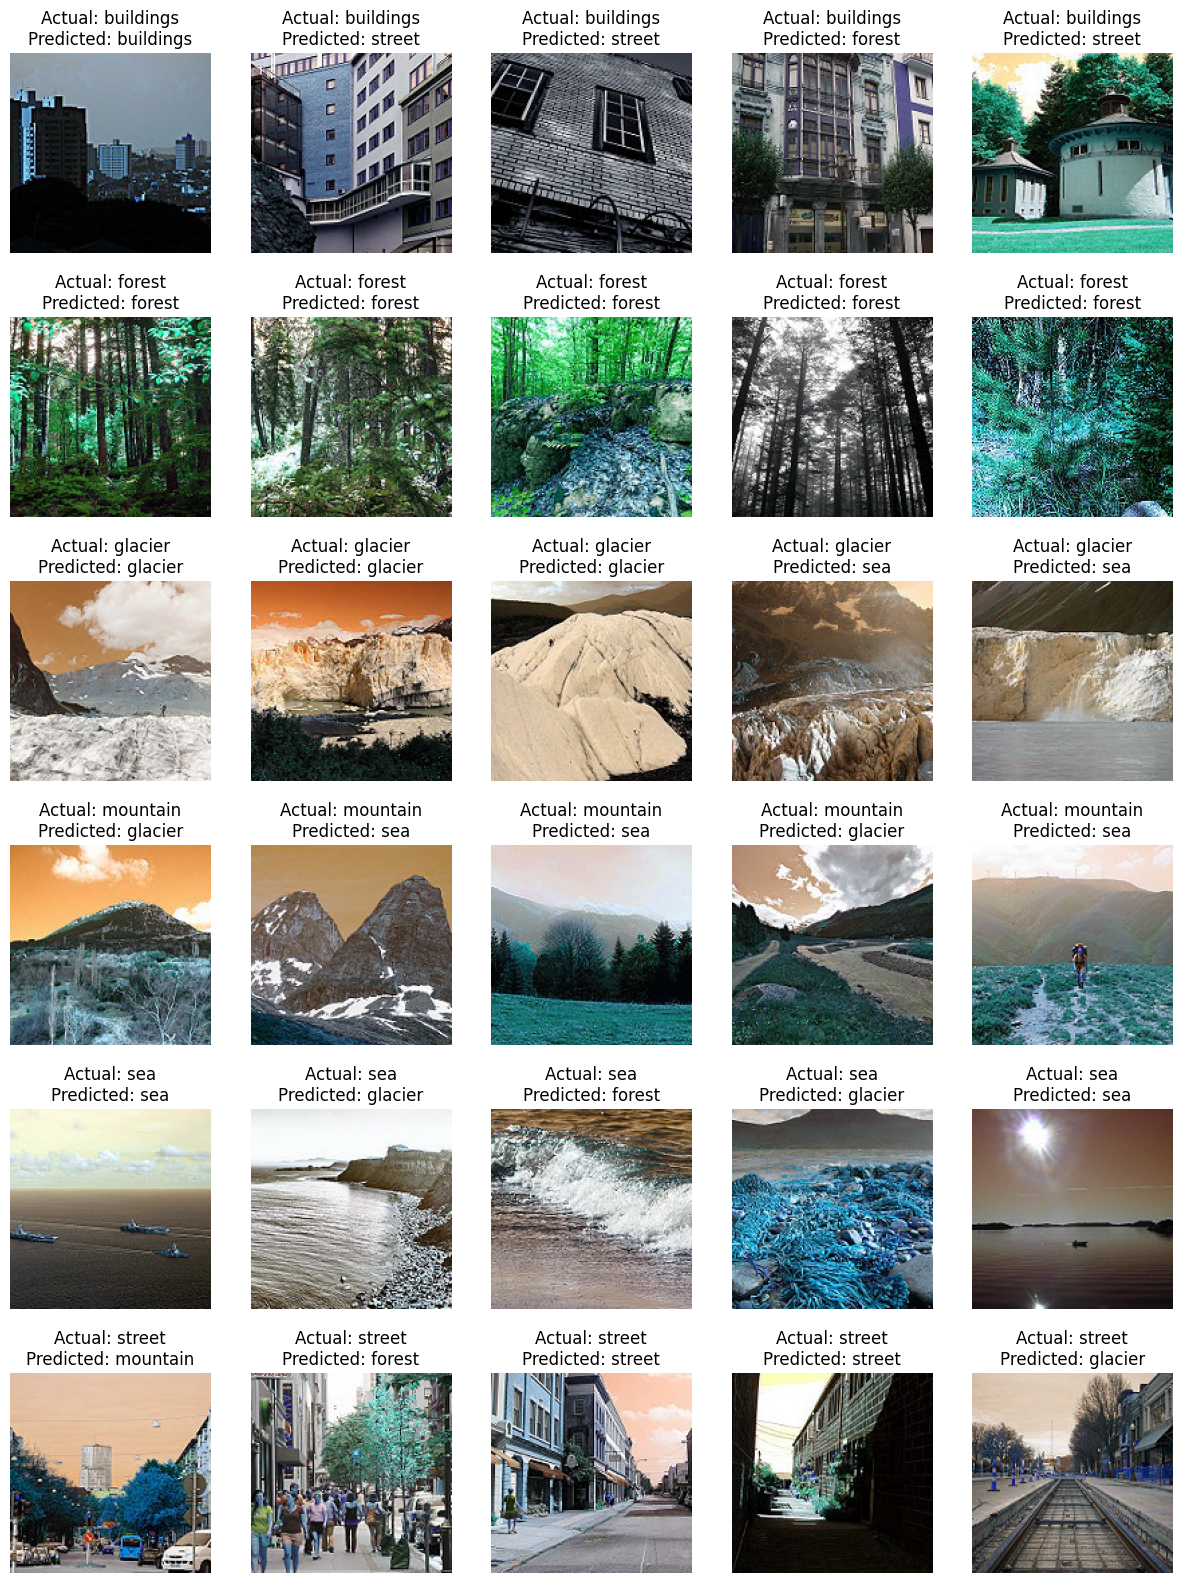
\includegraphics[width=1\linewidth]{images//ResNet50/TestingExamplesResNet.png}
    \caption{Testing Examples for ResNet50}
    \label{fig:Examples_ResNet}
\end{figure}

\subsubsection{DenseNet121}

The DenseNet121 technique has proven to be exceptionally effective, surpassing our expectations as the best-performing method thus far in our image classification endeavors. It has consistently demonstrated high accuracy and robustness across a wide range of classes, showcasing its capability to learn intricate patterns and features within the data.

\begin{figure}[H]
    \centering
    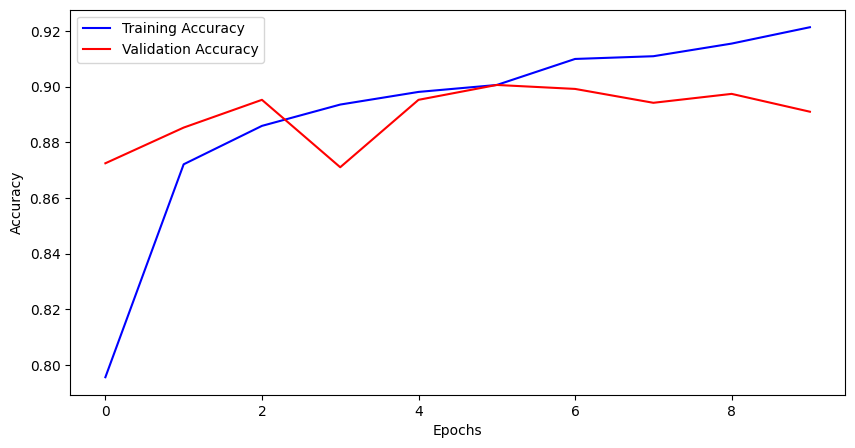
\includegraphics[width=1\linewidth]{images//DenseNet/TrainingValidationAccuracyDensenet.png}
    \caption{Training and Validation Accuracy for DenseNet121}
    \label{fig:TV_Accuracy_DenseNet}
\end{figure}

Despite its overall success, challenges persist in accurately distinguishing between certain classes, notably glaciers versus mountains and buildings versus streets. These distinctions pose significant difficulties due to the subtle visual similarities and varying environmental contexts present in the images.

\begin{figure}[H]
    \centering
    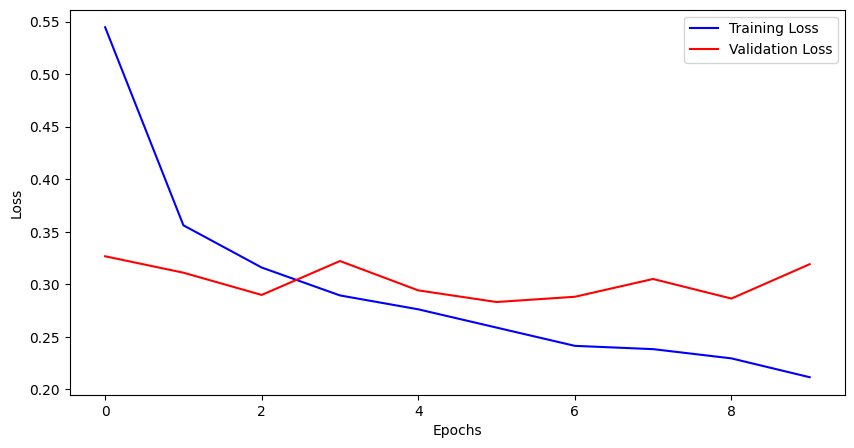
\includegraphics[width=1\linewidth]{images//DenseNet/TrainingValidationLossDenseNet.png}
    \caption{Training and Validation Loss for DenseNet121}
    \label{fig:TV_Accuracy_DenseNet}
\end{figure}

\begin{table}[H]
\centering
\begin{tabular}{lcccc}
\toprule
\textbf{} & \textbf{precision} & \textbf{recall} & \textbf{f1-score} & \textbf{support} \\
\midrule
buildings & 0.94 & 0.83 & 0.88 & 437 \\
forest & 0.99 & 0.99 & 0.99 & 474 \\
glacier & 0.81 & 0.88 & 0.84 & 553 \\
mountain & 0.85 & 0.82 & 0.83 & 525 \\
sea & 0.94 & 0.90 & 0.92 & 510 \\
street & 0.87 & 0.96 & 0.91 & 501 \\
\midrule
accuracy & & & 0.89 & 3000 \\
macro avg & 0.90 & 0.90 & 0.90 & 3000 \\
weighted avg & 0.90 & 0.89 & 0.89 & 3000 \\
\bottomrule
\end{tabular}
\caption{Performance metrics for DenseNet121}
\end{table}

\begin{figure}[H]
    \centering
    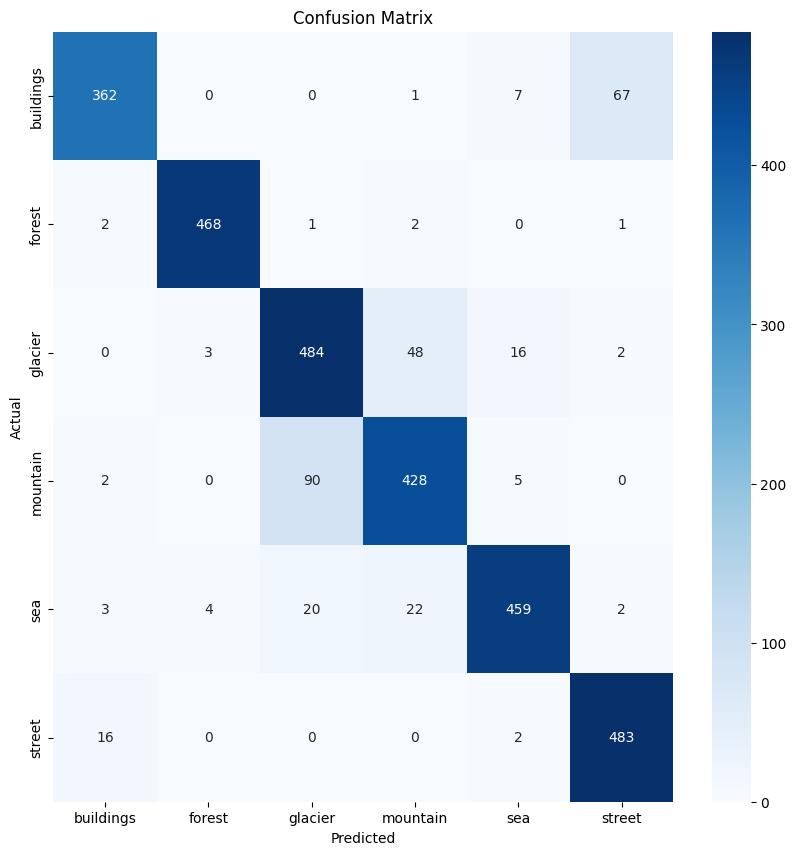
\includegraphics[width=1\linewidth]{images//DenseNet/ConfusionMatrixDenseNet.png}
    \caption{Confusion Matrix for DenseNet121}
    \label{fig:CM_DenseNet}
\end{figure}

To address these challenges head-on, we have decided to implement data augmentation techniques. By augmenting our training dataset with variations such as rotations, flips, and color adjustments, we aim to expose the model to a more diverse range of scenarios. This approach is crucial as it helps the model generalize better and learn more discriminative features that can distinguish between similar-looking classes more effectively.

Moreover, the application of data augmentation is expected to enhance the model's ability to handle variability and improve its overall accuracy in challenging classification tasks. We anticipate that this strategy will mitigate the errors observed in distinguishing glaciers versus mountains and buildings versus streets, ultimately refining our model's performance and reliability in real-world applications.

\begin{figure}[H]
    \centering
    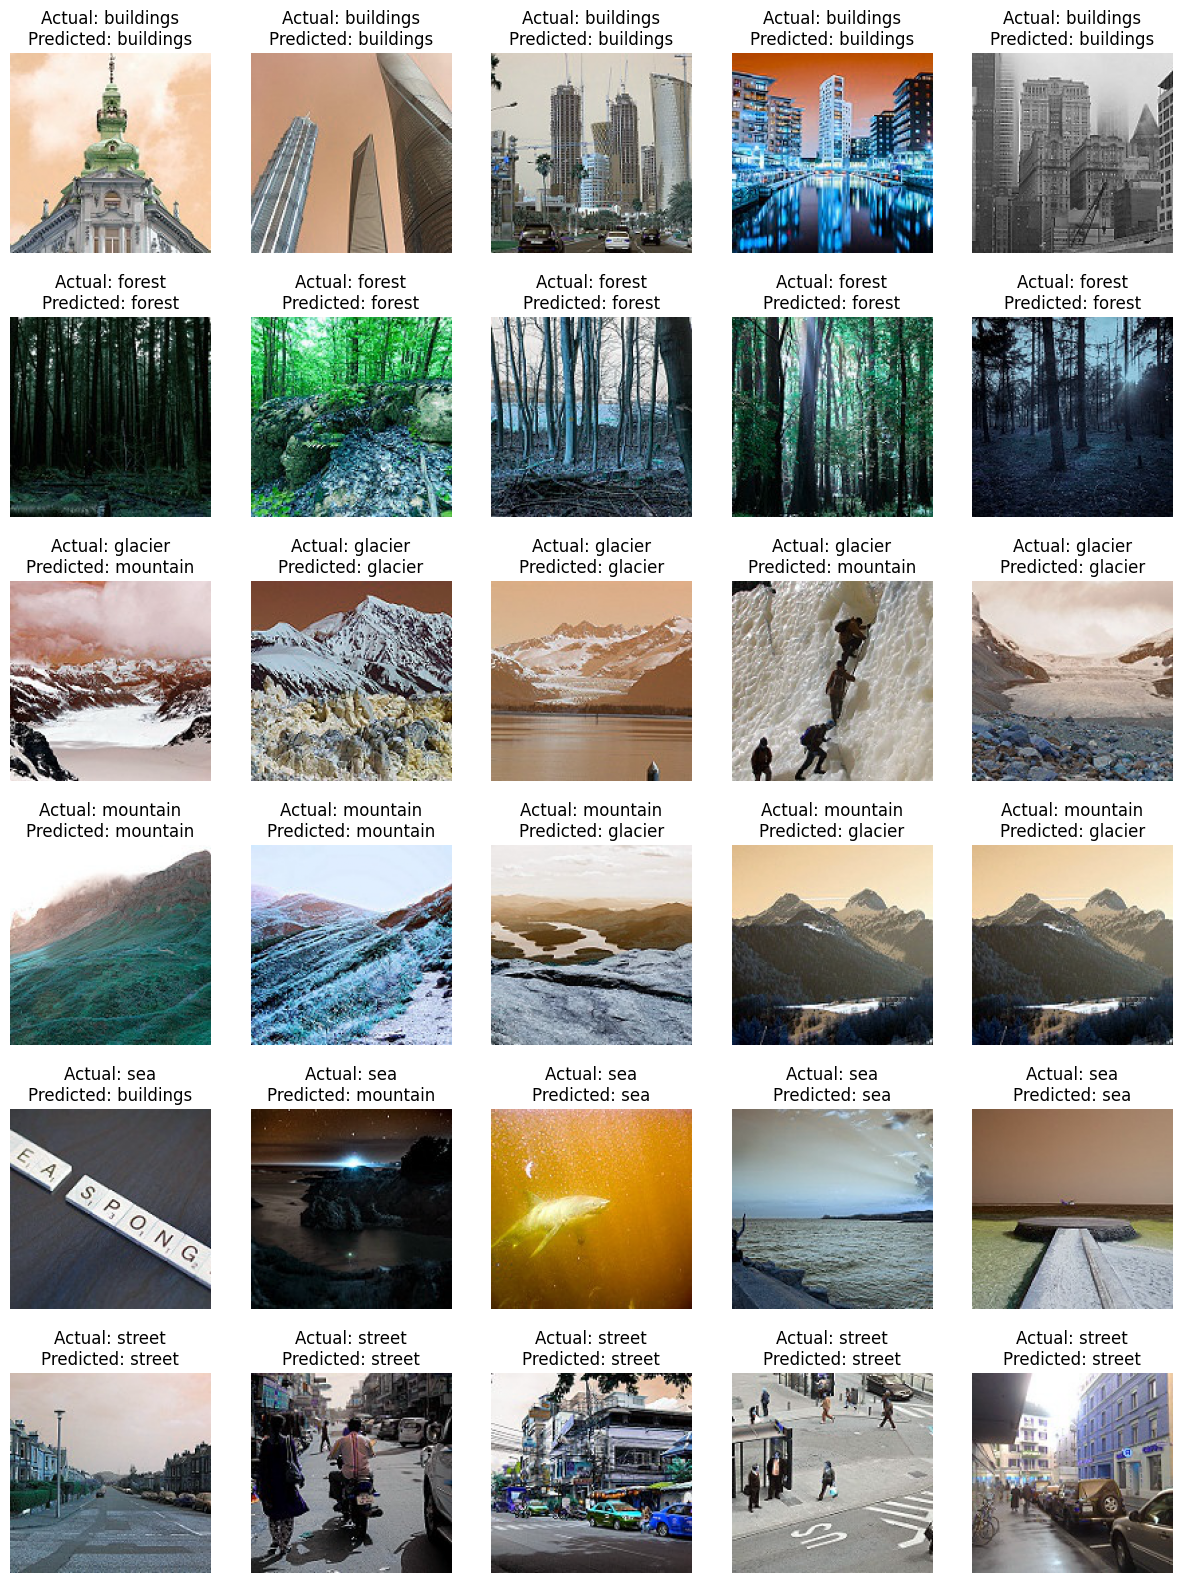
\includegraphics[width=1\linewidth]{images//DenseNet/TestingExamplesDenseNet.png}
    \caption{Testing Examples for DenseNet121}
    \label{fig:Examples_DenseNet}
\end{figure}

\subsubsection{DenseNet121 with augmented data}

With the implementation of data augmentation, we have observed significant improvements across various performance metrics of the model. Increasing the amount of training data has enhanced the model's generalization and robustness, resulting in improvements in accuracy, recall, and F1-score metrics. However, it is important to note that despite these advancements, the primary challenge of distinguishing between the classes of glaciers versus mountains and buildings versus streets persists. 

\begin{figure}[H]
    \centering
    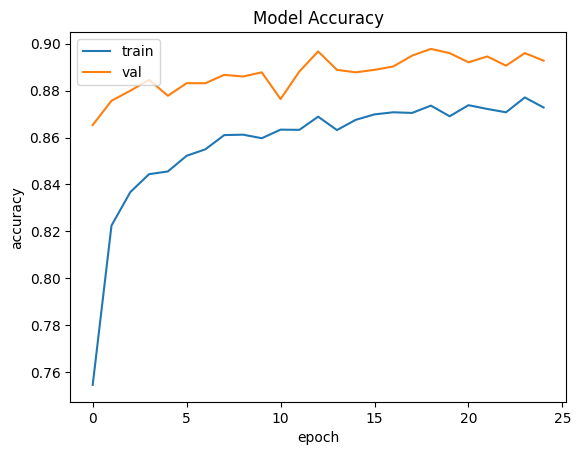
\includegraphics[width=1\linewidth]{images//DenseNet/Tranning_Validation_Accuracy_Densenet_Data_Augmented.png}
    \caption{Training and Validation Accuracy for DenseNet121 with Data Augmentation}
    \label{fig:TV_Accuracy_DenseNet_DA}
\end{figure}

\begin{figure}[H]
    \centering
    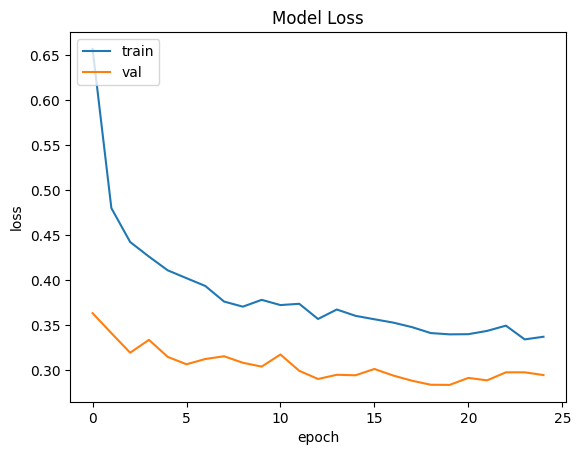
\includegraphics[width=1\linewidth]{images//DenseNet/Traning_Validation_Loss_DenseNet_Data_Augmented.png}
    \caption{Training and Validation Accuracy for DenseNet121 with Data Augmentation}
    \label{fig:TV_Loss_DenseNet_DA}
\end{figure}

\begin{table}[H]
\centering
\begin{tabular}{lcccc}
\toprule
\textbf{} & \textbf{precision} & \textbf{recall} & \textbf{f1-score} & \textbf{support} \\
\midrule
buildings & 0.94 & 0.86 & 0.90 & 437 \\
forest & 0.98 & 0.99 & 0.99 & 474 \\
glacier & 0.88 & 0.80 & 0.84 & 553 \\
mountain & 0.83 & 0.84 & 0.84 & 525 \\
sea & 0.89 & 0.95 & 0.92 & 510 \\
street & 0.89 & 0.95 & 0.92 & 501 \\
\midrule
accuracy & & & 0.90 & 3000 \\
macro avg & 0.90 & 0.90 & 0.90 & 3000 \\
weighted avg & 0.90 & 0.90 & 0.90 & 3000 \\
\bottomrule
\end{tabular}
\caption{Performance metrics for DenseNet121 with Data Augmentation}
\end{table}

\begin{figure}[H]
    \centering
    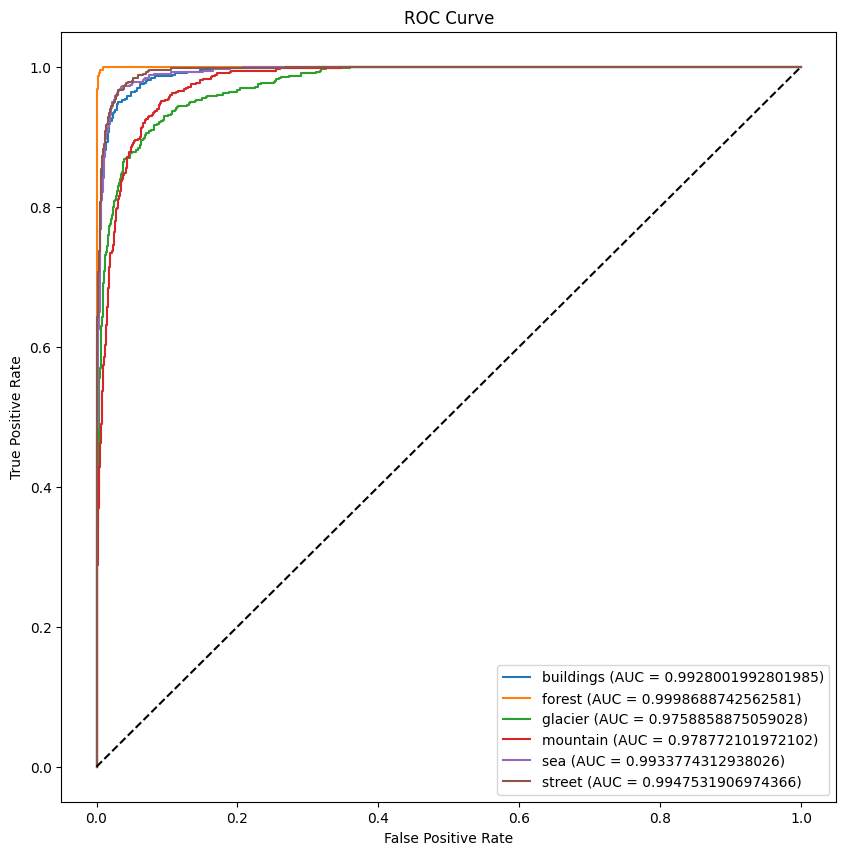
\includegraphics[width=1\linewidth]{images//DenseNet/ROC_DenseNet_Data_Augmented.png}
    \caption{ROC Curve for DenseNet121 with Data Augmentation}
    \label{fig:ROC_DenseNet_DA}
\end{figure}

This underscores the inherent complexity of similar images and emphasizes the ongoing need for model refinement and adjustments to achieve even higher accuracy.


\begin{figure}[H]
    \centering
    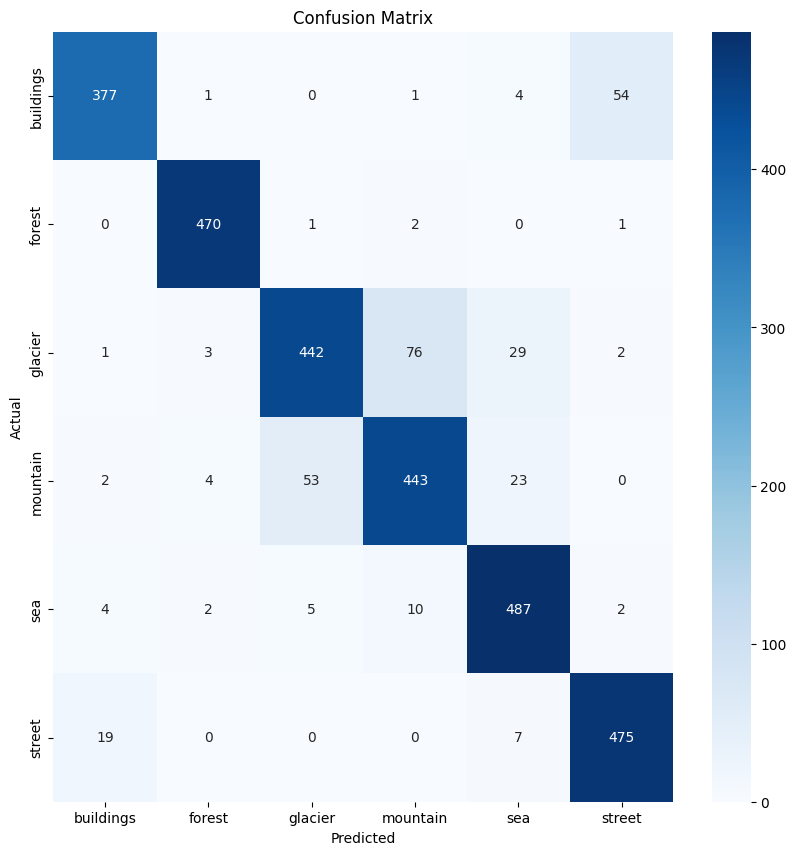
\includegraphics[width=1\linewidth]{images//DenseNet/ConfusionMatrix_DenseNet_Data_Augmented.png}
    \caption{Confusion Matrix for DenseNet121 with Data Augmentation}
    \label{fig:CM_Desenet_DA}
\end{figure}


\begin{figure}[H]
    \centering
    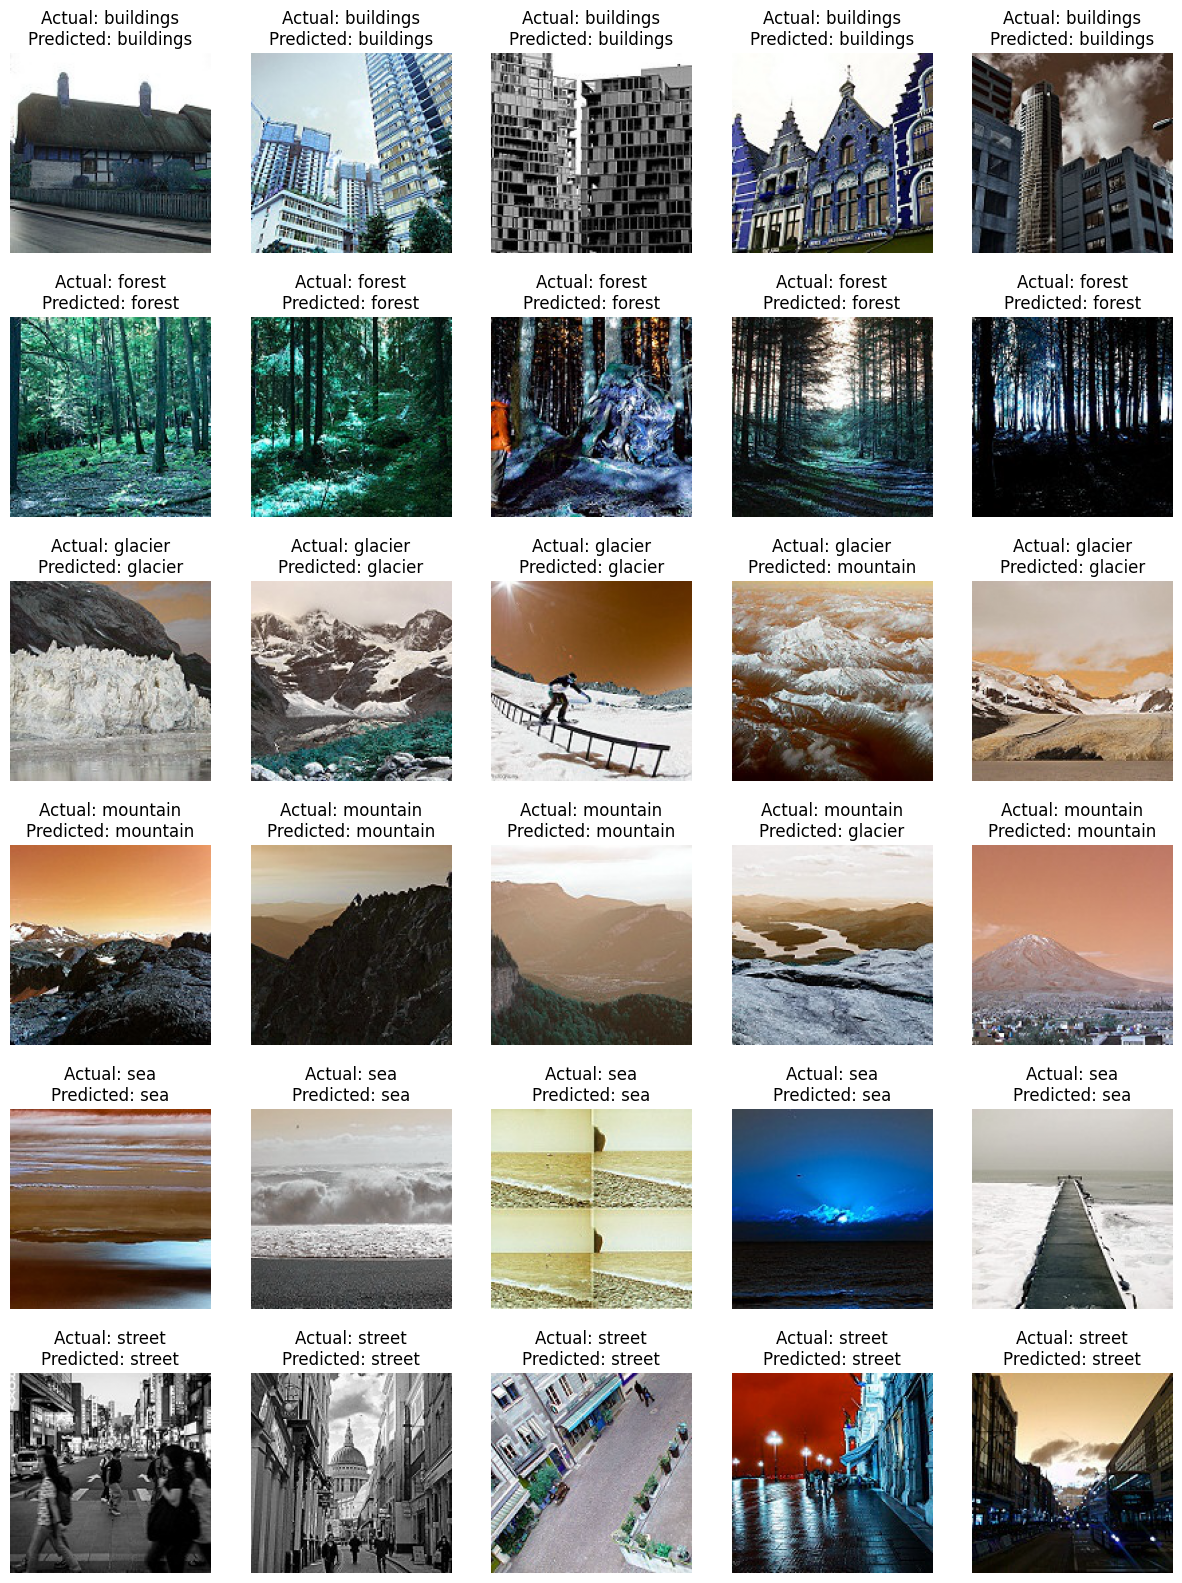
\includegraphics[width=1\linewidth]{images//DenseNet/Examples_DenseNet_DA.png}
    \caption{Testing Examples for DenseNet121 with Data Augmentation}
    \label{fig:enter-label}
\end{figure}

\subsubsection{VGG16}

The VGG16 technique has demonstrated respectable results in our experiments, although it hasn't surpassed some of our earlier methods. While it performs adequately overall, it does exhibit larger errors, particularly in distinguishing between the classes of glaciers and mountains. Despite its deep architecture and promising features, VGG16 seems to struggle with capturing the subtle distinctions between these visually similar categories.

\begin{figure}[H]
    \centering
    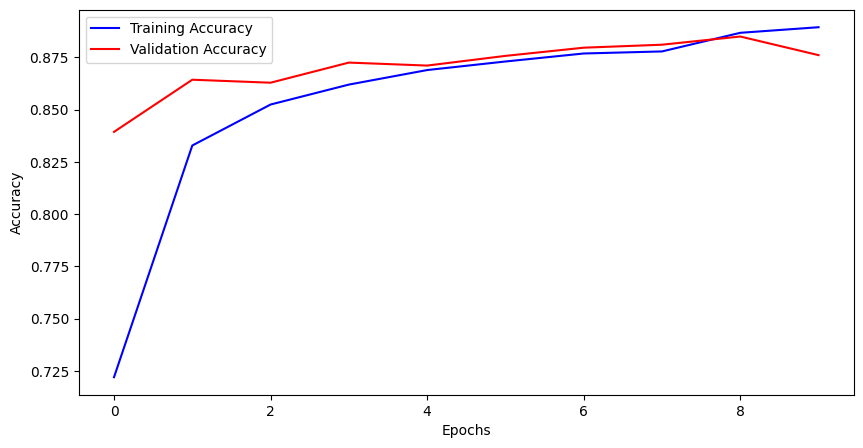
\includegraphics[width=1\linewidth]{images//VGG16/Testing_Validation_Accuracy_VGG16.png}
    \caption{Training and Validation Accuracy for VGG16}
    \label{fig:TV_Accuracy_VGG16}
\end{figure}


\begin{figure}[H]
    \centering
    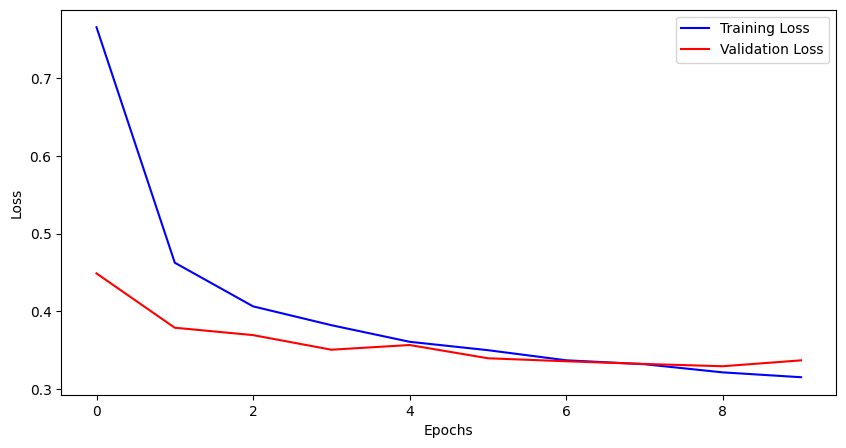
\includegraphics[width=1\linewidth]{images//VGG16/Training_Validation_Loss_VGG16.png}
    \caption{Training and Validation Loss for VGG16}
    \label{fig:TV_Loss_VGG16}
\end{figure}

\begin{table}[H]
\centering
\begin{tabular}{lcccc}
\toprule
\textbf{} & \textbf{precision} & \textbf{recall} & \textbf{f1-score} & \textbf{support} \\
\midrule
buildings & 0.89 & 0.90 & 0.89 & 437 \\
forest & 0.97 & 0.99 & 0.98 & 474 \\
glacier & 0.88 & 0.73 & 0.80 & 553 \\
mountain & 0.79 & 0.87 & 0.83 & 525 \\
sea & 0.86 & 0.93 & 0.89 & 510 \\
street & 0.91 & 0.88 & 0.90 & 501 \\
\midrule
accuracy & & & 0.88 & 3000 \\
macro avg & 0.88 & 0.88 & 0.88 & 3000 \\
weighted avg & 0.88 & 0.88 & 0.88 & 3000 \\
\bottomrule
\end{tabular}
\caption{Performance metrics for VGG16}
\end{table}

\begin{figure}[H]
    \centering
    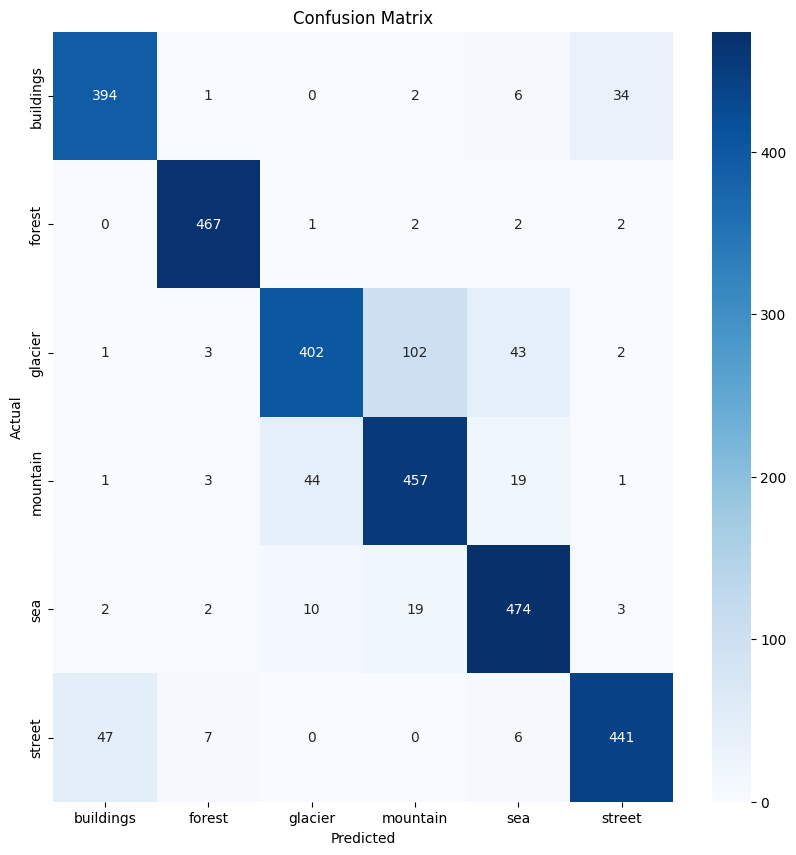
\includegraphics[width=1\linewidth]{images//VGG16/ConfusionMatrixVGG16.png}
    \caption{Confusion Matrix for VGG16}
    \label{fig:CM_VGG16}
\end{figure}

Our evaluation reveals that VGG16 achieves competitive performance in terms of accuracy and generalization across other classes but consistently encounters challenges with these specific distinctions. This highlights a persistent issue in image classification tasks where certain classes, such as glaciers versus mountains, pose greater difficulty due to their visual similarities and varying environmental conditions.

In conclusion, while VGG16 has shown promise in various aspects of our classification task, including general performance across diverse classes, mitigating errors in critical distinctions such as glaciers versus mountains remains a priority for achieving more robust and accurate results.

\begin{figure}[H]
    \centering
    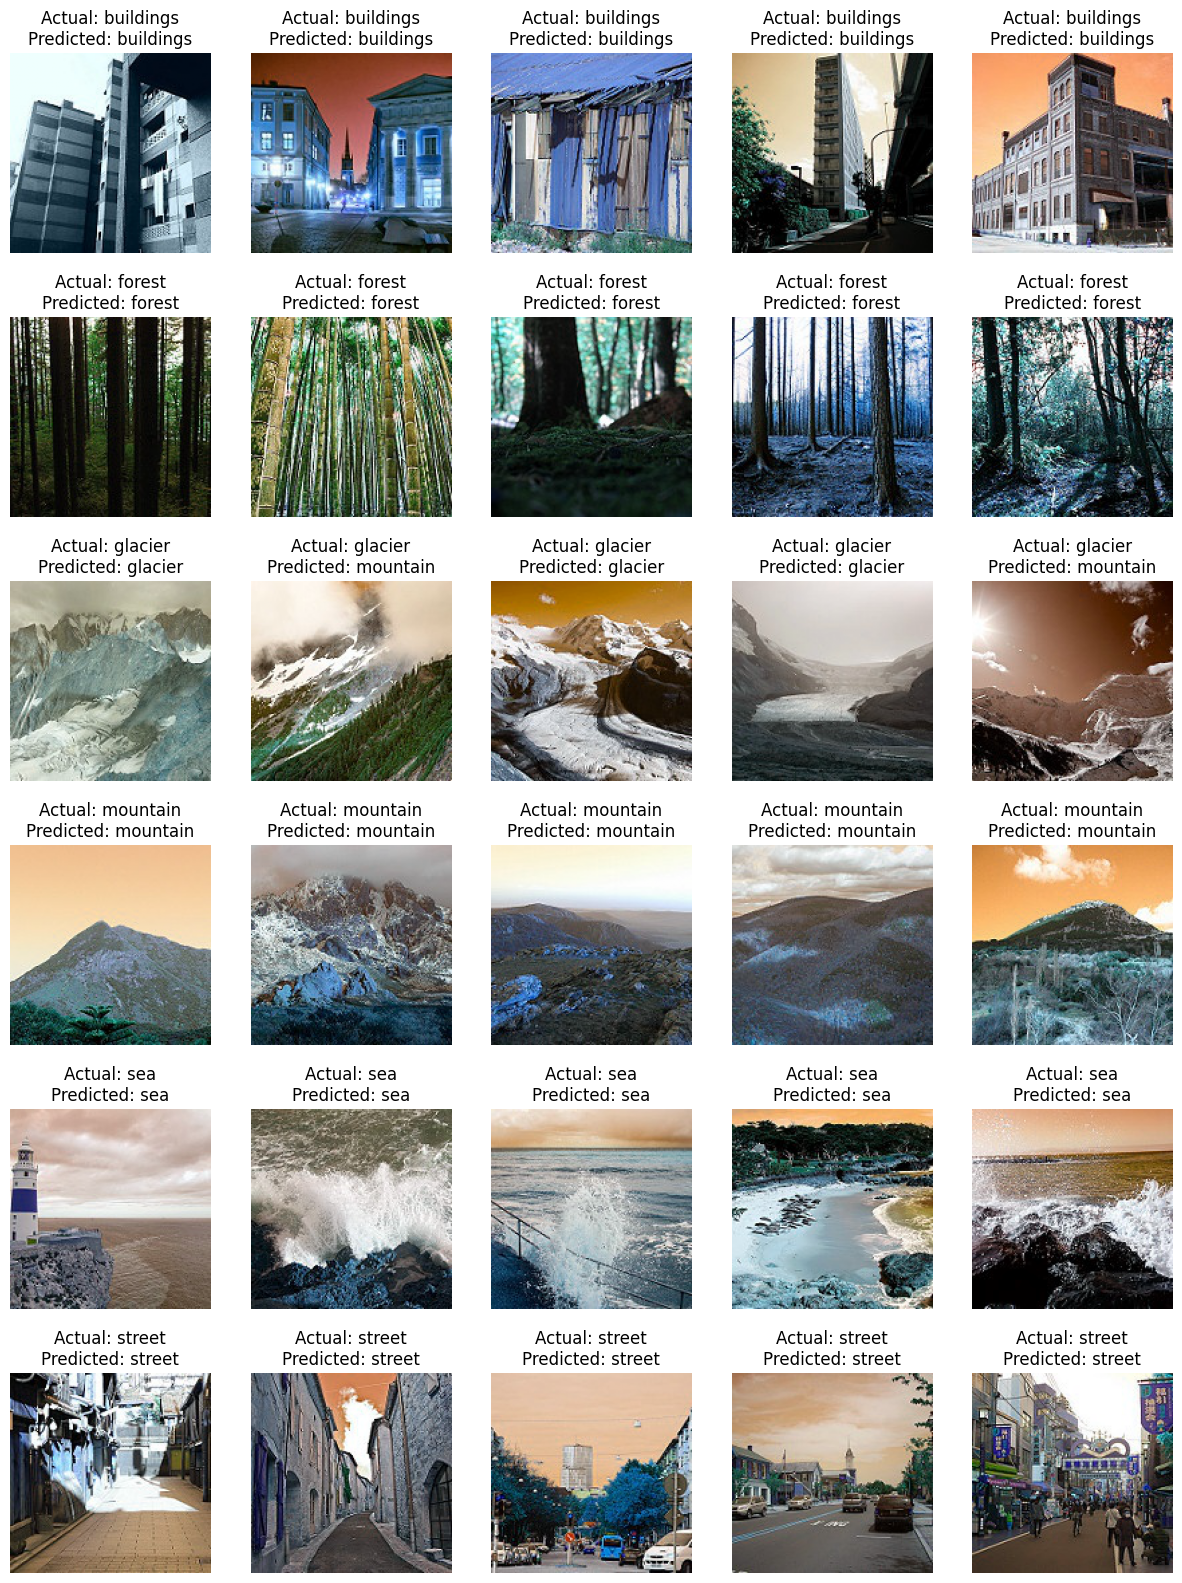
\includegraphics[width=1\linewidth]{images//VGG16/ExamplesVGG16.png}
    \caption{Testing Examples for VGG16}
    \label{fig:ExamplesVGG16}
\end{figure}

\subsubsection{VGG16 With Data Augmentation}

Introducing data augmentation significantly enhanced the performance of the VGG16 model in our experiments. This augmentation strategy involves applying various transformations like rotations, flips, and shifts to training images, which effectively boosted the model's ability to generalize across different classes. The augmented VGG16 model demonstrates improved accuracy and robustness in distinguishing between visually similar categories such as glaciers and mountains, showcasing its enhanced capability to handle complex image distinctions with greater precision.

Additionally, it's worth noting that among our models evaluated, VGG16 with data augmentation stood out as the third best performer overall. This ranking highlights its substantial improvement over baseline methods, reflecting its enhanced ability to learn intricate patterns and generalize effectively across diverse datasets.

\begin{figure}[H]
    \centering
    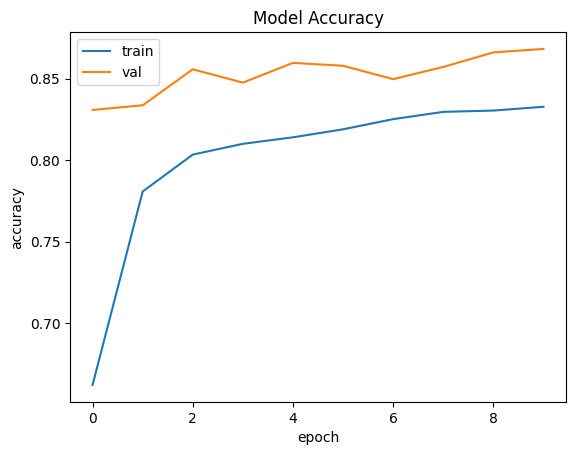
\includegraphics[width=1\linewidth]{images//VGG16/Training_Validation_Accuracy_VGG16_Data_Augmented.png}
    \caption{Training and Validation Accuracy for VGG16 with Data Augmentation}
    \label{fig:TV_VGG16_DA}
\end{figure}

\begin{figure}[H]
    \centering
    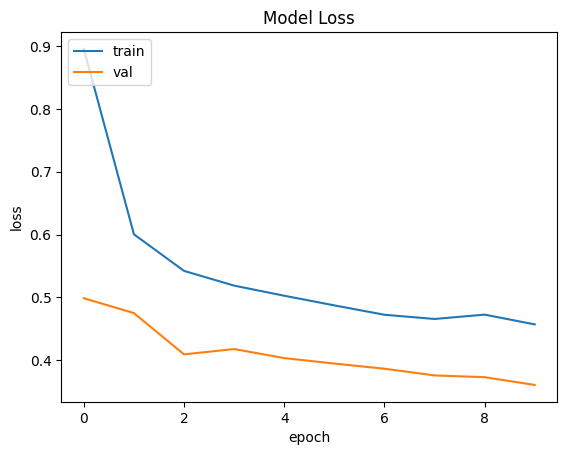
\includegraphics[width=1\linewidth]{images//VGG16/Training_Validation_Loss_VGG16_Data_Augmented.png}
    \caption{Training and Validation Loss for VGG16 with Data Augmentation}
    \label{fig:TV_Loss_VGG16_DA}
\end{figure}

\begin{table}[H]
\centering
\begin{tabular}{lcccc}
\toprule
\textbf{} & \textbf{precision} & \textbf{recall} & \textbf{f1-score} & \textbf{support} \\
\midrule
buildings & 0.87 & 0.89 & 0.88 & 437 \\
forest & 0.97 & 0.96 & 0.96 & 474 \\
glacier & 0.78 & 0.85 & 0.81 & 553 \\
mountain & 0.82 & 0.80 & 0.81 & 525 \\
sea & 0.90 & 0.84 & 0.87 & 510 \\
street & 0.89 & 0.88 & 0.88 & 501 \\
\midrule
accuracy & & & 0.87 & 3000 \\
macro avg & 0.87 & 0.87 & 0.87 & 3000 \\
weighted avg & 0.87 & 0.87 & 0.87 & 3000 \\
\bottomrule
\end{tabular}
\caption{Performance metrics for VGG16 with Data Augmentation}
\end{table}


\begin{figure}[H]
    \centering
    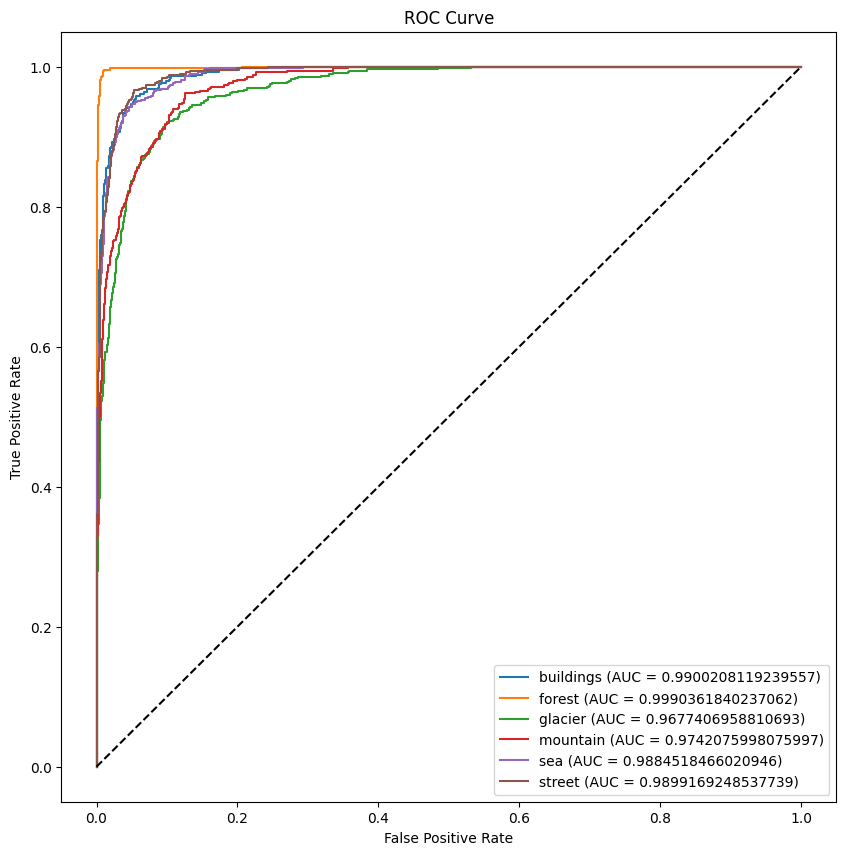
\includegraphics[width=1\linewidth]{images//VGG16/ROC_VGG16_DA.png}
    \caption{ROC Curve for VGG16 with Data Augmentation}
    \label{fig:ROC_VGG_DA}
\end{figure}

Compared to the model without data augmentation, this augmented VGG16 model demonstrates enhanced capability in distinguishing between glaciers and mountains, as depicted in the confusion matrix below

\begin{figure}[H]
    \centering
    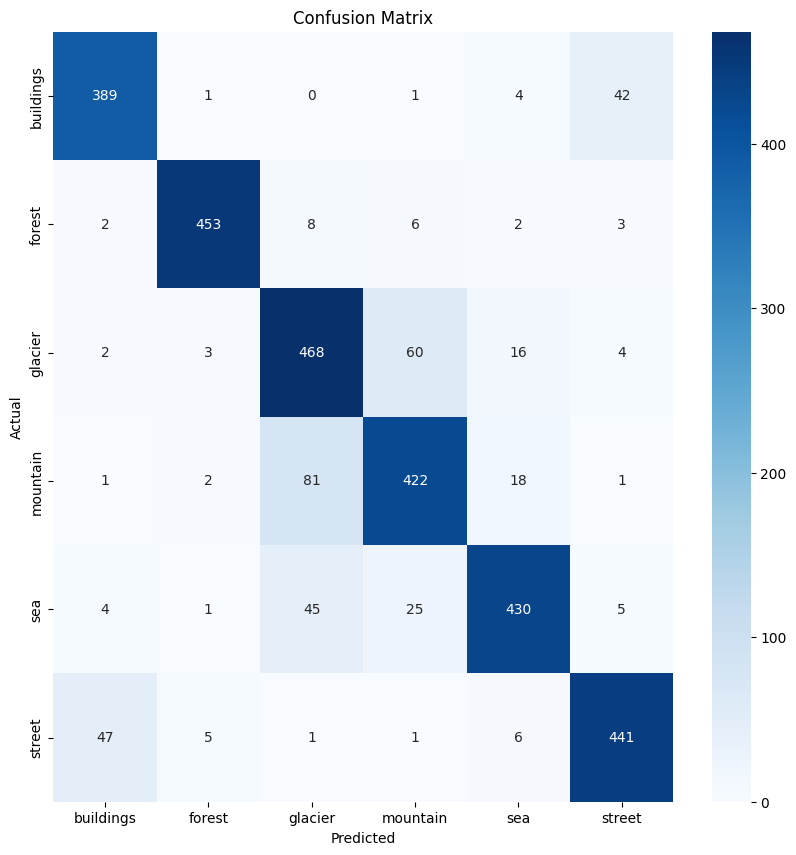
\includegraphics[width=1\linewidth]{images//VGG16/CM_VGG1&_DA.png}
    \caption{Confusion Matrix for VGG16 with Data Augmentation}
    \label{fig:CM_VGG_Da}
\end{figure}

\begin{figure}[H]
    \centering
    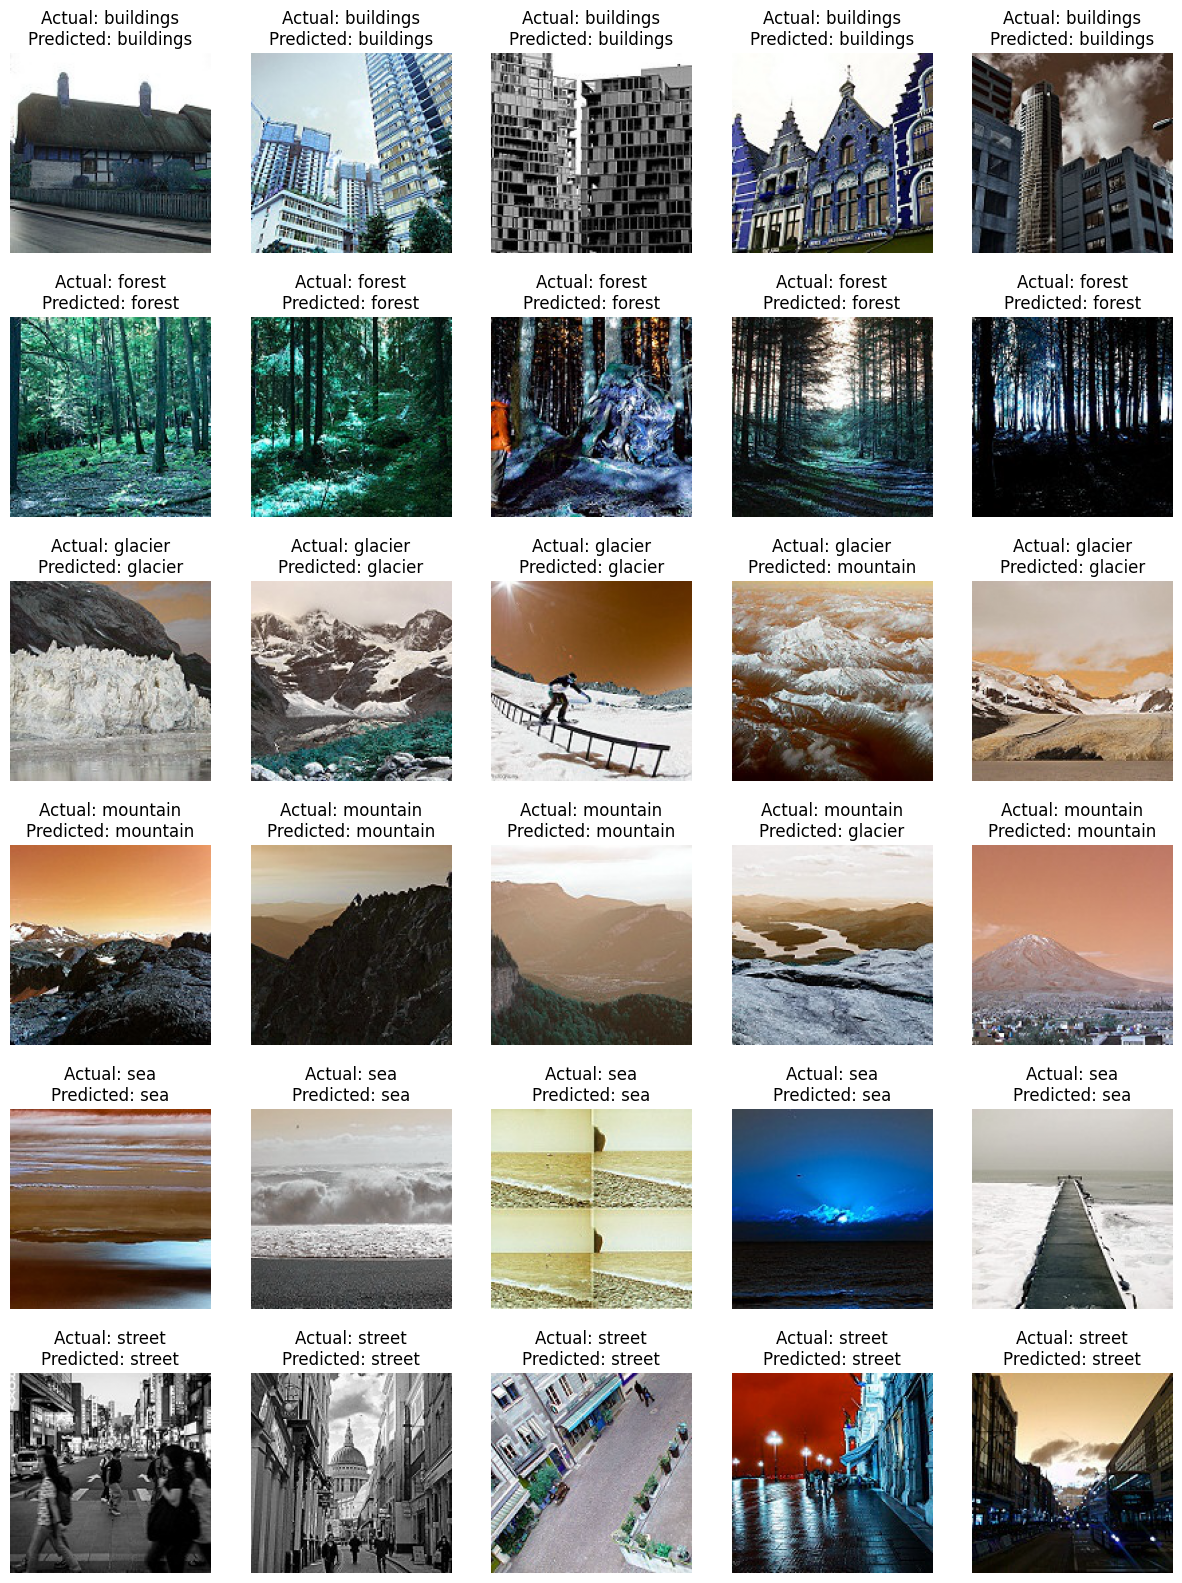
\includegraphics[width=1\linewidth]{images//VGG16/Examples_VGG16_DA.png}
    \caption{Testing Examples for VGG16 with Data Augmentation}
    \label{fig:Examples_VGG_DA}
\end{figure}

\subsection{Results analysis}

\section{Comparing Results With State of Art}

\begin{table}[h]
\centering
\begin{tabular}{|l|l|}
\hline
\textbf{Notebook} & \textbf{Accuracy} \\ \hline
Ours & 90\% \\ \hline
Transfer Learning With Keras - VGG16 / VGG19 & 89.3\% \\ \hline
[BEG][TUT] Intel Image Classification [93.76\% Accur] & 93.76\% \\ \hline
Intel Image Classification (CNN - Keras) & 87.8\% \\ \hline
Intel Images Classification by CNN & 82.4\% \\ \hline
Image Classification using CNN & 94.3\% \\ \hline
\end{tabular}
\label{table}
\end{table}

This comparisons are not the fairest ones, since all the works use different transformations of the dataset. Due to the computation capacity that we had available, we did not use most of the classes and our results should be compared with that in mind. Nevertheless, we were able to achieve good results and to present an interesting work, which could give future researches on the dataset a starting point.

\section{Conclusion}

Our recent venture into the realm of machine learning marked a significant milestone, enriching our expertise in this evolving field and deepening our appreciation for its intricacies. This project not only met our primary objectives but also provided valuable insights that extended beyond our initial goals, serving as a comprehensive study in the domain. Our exploration encompassed various strategies, with a notable emphasis on convolutional neural networks (CNNs), which not only clarified concepts previously muddled by class materials but also required a deeper understanding to navigate effectively.

Overall, the outcomes were undeniably positive, bolstering our confidence in tackling future challenges within this burgeoning field. This experience has undoubtedly broadened our horizons, cementing machine learning as an integral part of our professional journey moving forward.

Furthermore, it was not feasible to perform hyperparameter tuning across different models due to execution time constraints. However, we acknowledge the significance of this practice and note that examples and hyperparameter tuning techniques are available in our Jupyter notebook. Drawing from our prior experience, including our first project where we explored these methods, we deem it non-critical for this specific project. Nevertheless, we recognize that such tuning could potentially enhance the outcomes achieved.

\section{Work Load}

Each student worked 50\% of the project.

\section{Acknowledgment}

The authors would like to thank professor Petia Georgieva, regent of TAA course, for her support, assistance throughout the project and the flexibility for the project delivery date.

\bibliographystyle{unsrt}
\begin{thebibliography}{10}

\bibitem{boser1992training}
Boser, B. E., Guyon, I. M., \& Vapnik, V. N. (1992).
A training algorithm for optimal margin classifiers.
\textit{Proceedings of the fifth annual workshop on Computational learning theory} (pp. 144-152).

\bibitem{breiman2001random}
Breiman, L. (2001).
Random forests.
\textit{Machine learning}, 45(1), 5-32.

\bibitem{krizhevsky2012imagenet}
Krizhevsky, A., Sutskever, I., \& Hinton, G. E. (2012).
ImageNet classification with deep convolutional neural networks.
\textit{Advances in neural information processing systems}, 25.

\bibitem{simonyan2014very}
Simonyan, K., \& Zisserman, A. (2014).
Very deep convolutional networks for large-scale image recognition.
\textit{arXiv preprint arXiv:1409.1556}.

\bibitem{he2016deep}
He, K., Zhang, X., Ren, S., \& Sun, J. (2016).
Deep residual learning for image recognition.
\textit{Proceedings of the IEEE conference on computer vision and pattern recognition} (pp. 770-778).

\bibitem{huang2017densely}
Huang, G., Liu, Z., Van Der Maaten, L., \& Weinberger, K. Q. (2017).
Densely connected convolutional networks.
\textit{Proceedings of the IEEE conference on computer vision and pattern recognition} (pp. 4700-4708).

\bibitem{sharif2014cnn}
Sharif Razavian, A., Azizpour, H., Sullivan, J., \& Carlsson, S. (2014).
CNN features off-the-shelf: an astounding baseline for recognition.
\textit{Proceedings of the IEEE conference on computer vision and pattern recognition workshops} (pp. 806-813).

\bibitem{srivastava2014dropout}
Srivastava, N., Hinton, G., Krizhevsky, A., Sutskever, I., \& Salakhutdinov, R. (2014).
Dropout: A simple way to prevent neural networks from overfitting.
\textit{The journal of machine learning research}, 15(1), 1929-1958.

\bibitem{b8} 
SVC. [Online]. Available: \url{https://scikit-learn.org/stable/modules/generated/sklearn.svm.SVC.html}

\bibitem{b9} 
Validation curve explanation. [Online]. Available: \url{https://www.geeksforgeeks.org/validation-curve/}

\bibitem{b10} 
Train Test function from sklearn. [Online]. Available: \url{https://scikit-learn.org/stable/modules/generated/sklearn.model_selection.train_test_split.html}

\bibitem{b11} 
StandardScaler. [Online]. Available: \url{https://scikit-learn.org/stable/modules/generated/sklearn.preprocessing.StandardScaler.html}

\bibitem{b12} 
Confusion matrix function from sklearn. [Online]. Available: \url{https://scikit-learn.org/stable/modules/generated/sklearn.metrics.confusion_matrix.html}

\bibitem{b13} 
Logistic Regression Definition. [Online]. Available: \url{https://ml-cheatsheet.readthedocs.io/en/latest/logistic_regression.html}

\bibitem{b14} 
Precision score function from sklearn. [Online]. Available: \url{https://scikit-learn.org/stable/modules/generated/sklearn.metrics.precision_score.html}

\bibitem{b15} 
Hyperparameter tuning definition. [Online]. Available: \url{https://www.jeremyjordan.me/hyperparameter-tuning/}

\bibitem{b16} 
Gradient Boosting Regressor. [Online]. Available: \url{https://scikit-learn.org/stable/modules/generated/sklearn.ensemble.GradientBoostingRegressor.html}

\bibitem{b17} 
Hyper-parameter tuning. [Online]. Available: \url{https://scikit-learn.org/stable/modules/grid_search.html}

\bibitem{b18} 
Subsampling For Class Imbalances. [Online]. Available: \url{https://topepo.github.io/caret/subsampling-for-class-imbalances.html}

\bibitem{b19} 
Neural Network. [Online]. Available: \url{https://scikit-learn.org/stable/modules/neural_networks_supervised.html}

\bibitem{b20} 
F1 score function from sklearn. [Online]. Available: \url{https://scikit-learn.org/stable/modules/generated/sklearn.metrics.f1_score.html}

\bibitem{b21} 
K-fold. [Online]. Available: \url{https://scikit-learn.org/stable/modules/cross_validation.html}

\bibitem{b22} 
Correlation Matrix. [Online]. Available: \url{https://datatofish.com/correlation-matrix-pandas/}

\bibitem{b23} 
Recall score function from sklearn. [Online]. Available: \url{https://scikit-learn.org/stable/modules/generated/sklearn.metrics.recall_score.html}

\bibitem{b24} 
Logistic Regression. [Online]. Available: \url{https://scikit-learn.org/stable/modules/generated/sklearn.linear_model.LogisticRegression.html/}

\bibitem{b25} 
Confusion Matrix Example. [Online]. Available: \url{https://sairampenjarla.medium.com/sensitivity-and-specificity-in-machine-learning-3af012fbe488}

\bibitem{b26} 
Learning Curve Example. [Online]. Available: \url{https://medium.com/@singh.santosh2702/ann-model-testing-and-training-accuracy-using-keras-and-tensorflow-c9c2e1a1b7df}

\bibitem{notebook1}
Transfer Learning With Keras - VGG16 / VGG19. 
Retrieved from \url{https://www.kaggle.com/code/ihsncnkz/transfer-learning-with-keras-vgg16-vgg19}.

\bibitem{notebook2}
[BEG][TUT]Intel Image Classification[93.76\% Accur]. 
Retrieved from \url{https://www.kaggle.com/code/uzairrj/beg-tut-intel-image-classification-93-76-accur}.

\bibitem{notebook3}
Intel Image Classification (CNN - Keras). 
Retrieved from \url{https://www.kaggle.com/code/vincee/intel-image-classification-cnn-keras}.

\bibitem{notebook4}
Intel Images Classification by CNN. 
Retrieved from \url{https://www.kaggle.com/code/bibo600/intel-images-classification-by-cnn}.

\bibitem{notebook5}
Image Classification using CNN. 
Retrieved from \url{https://www.kaggle.com/code/madhumithakolkar/image-classification-using-cnn}.

\bibitem{numpy}
NumPy. [Online]. Available: \url{https://numpy.org/}

\bibitem{pandas}
Pandas. [Online]. Available: \url{https://pandas.pydata.org/}

\bibitem{matplotlib}
Matplotlib. [Online]. Available: \url{https://matplotlib.org/}

\bibitem{seaborn}
Seaborn. [Online]. Available: \url{https://seaborn.pydata.org/}

\bibitem{imageDataGenerator}
Keras ImageDataGenerator. [Online]. Available: \url{https://keras.io/api/preprocessing/image/}

\bibitem{labelEncoder}
LabelEncoder from sklearn. [Online]. Available: \url{https://scikit-learn.org/stable/modules/generated/sklearn.preprocessing.LabelEncoder.html}

\bibitem{toCategorical}
Keras tocategorical. [Online]. Available: \url{https://keras.io/api/utils/python_utils/#to_categorical-function}

\bibitem{sequential}
Keras Sequential model. [Online]. Available: \url{https://keras.io/api/models/sequential/}

\bibitem{conv2d}
Keras Conv2D layer. [Online]. Available: \url{https://keras.io/api/layers/convolution_layers/convolution2d/}

\bibitem{maxPooling2d}
Keras MaxPooling2D layer. [Online]. Available: \url{https://keras.io/api/layers/pooling_layers/max_pooling2d/}

\bibitem{flatten}
Keras Flatten layer. [Online]. Available: \url{https://keras.io/api/layers/reshaping_layers/flatten/}

\bibitem{dense}
Keras Dense layer. [Online]. Available: \url{https://keras.io/api/layers/core_layers/dense/}

\bibitem{dropout}
Keras Dropout layer. [Online]. Available: \url{https://keras.io/api/layers/regularization_layers/dropout/}

\bibitem{vgg16image}
An overview of VGG16 and NiN models
\url{https://lekhuyen.medium.com/an-overview-of-vgg16-and-nin-models-96e4bf398484}

\bibitem{densenetarch}
MLT CNN Architectures: DenseNet - theory
\url{https://www.youtube.com/watch?v=wh-n-pTxMZU&ab_channel=MLTArtificialIntelligence}

\bibitem{Receiver operating characteristic}
Receiver operating characteristic
\url{https://en.wikipedia.org/wiki/Receiver_operating_characteristic}

\bibitem{UFPR}
Universidade Federal do Paraná (UFPR)
Especialização em Engenharia Industrial 4.0
\url{https://www.inf.ufpr.br/menotti/am-17/slides/ML-05class2.pdf}

\end{thebibliography}

\end{document}